%------------------------------------------------Main.tex % the one that you should compile ;)

\documentclass[a4paper,12pt,oneside]{report}

%------------------------------------------------packages

\usepackage[colorlinks=true, linkcolor=black]{hyperref} 
\usepackage{longtable}
\usepackage[square, numbers, comma, sort&compress]{natbib}
 \usepackage[french]{babel}
\usepackage{array,multirow,makecell}
\usepackage{setspace}
\usepackage{ulem}
\usepackage[utf8x]{inputenc}
\usepackage{amsmath}
\usepackage[table]{xcolor}
\definecolor{myblue}{RGB}{120,206,252}
\usepackage{booktabs}
\usepackage{adjustbox}
\usepackage{tikz}
\usetikzlibrary{arrows.meta, shapes.geometric}
\usepackage{float}
\usepackage{booktabs}
\usepackage{colortbl}
\usepackage{array}
\usepackage{makecell}

\usepackage{tikz}
\usetikzlibrary{arrows.meta, shapes, positioning, calc, fit, bending}


\definecolor{lightblue}{HTML}{00A6FF}
\hypersetup{
   colorlinks=true,
    citecolor=lightblue,
    filecolor=lightblue,
    urlcolor=lightblue
}


\definecolor{seopurple}{HTML}{006ca8}
\definecolor{seolightpurple}{HTML}{e9f5f6}
\definecolor{geoblue}{HTML}{003899}
\definecolor{geolightblue}{HTML}{e0e7f4}
\definecolor{rowgray}{HTML}{f4f4f4}
\definecolor{headertext}{HTML}{FFFFFF}
%------------------------- arabe text
\usepackage{arabtex}
\usepackage{utf8}
%-----------------------------------
\usepackage[T1]{fontenc}
\usepackage{graphicx}

\usepackage{titling}
%------ e9leb titre

\usepackage{adjustbox} 
\usepackage{blindtext}
%-----
\usepackage{url}
\usepackage{titlesec}
\usepackage{marvosym}
\usepackage{tabularx}
\usepackage[top=3cm,bottom=3cm,left=2cm,right=2cm]{geometry}
\usepackage{fancyhdr}
\usepackage{enumitem}
\usepackage{amsfonts}
\usepackage{soul}
\usepackage{xcolor}
\pagestyle{fancy}
\renewcommand{\headrulewidth}{2pt}
\newcommand{\horrule}[1]{\rule{\linewidth}{#1}} % Horizontal rule
\usepackage{pifont} %----for customized item label
\setlength{\headheight}{15pt} 
\usepackage{version}  %----to use \begin{comment}
\setlength{\parskip}{0.7em}   %--espace entre paragraphes
\usepackage{lettrine} %----first big letter 
\usepackage{indentfirst}
\usepackage{subcaption}
\usepackage{tcolorbox}

\usepackage{listings}

%---------------------------------------------------more packages
\usepackage{ulem}
\newcommand{\HRule}{\textcolor{lightgray}{\rule{15.5 cm}{0.12 cm}}}
\newcommand{\Hrule}{\textcolor{lightgray}{\rule{13.5 cm}{0.15 cm}}}



 \fancyhead[L]{}
 %\renewcommand{\footrulewidth}{0.4pt}
 %\fancyfoot[L]{Graduation Internship Report}
 %\fancyfoot[R]{2016 - 2017}
%-------------------- interligne
\renewcommand{\baselinestretch}{1.3}


\usepackage[section]{placeins}

%------------------------------format du titre de section
\titleformat{\section}[block]
  {\huge\bfseries}
  {\color{gray} \thesection
   \hspace{10pt}\vline}
  {10pt}
  {}


\newcommand{\customizeNumber}{%
  \fontsize{40}{40}\usefont{U}{eur}{b}{n}}

\newcommand{\chapterNumber}{%
  \fontsize{12}{12}\usefont{U}{b}{n}}



%---------------------------------------------Here We Go !
\begin{document}

\selectlanguage{english}

{
\setcounter{tocdepth}{3}
\setcounter{secnumdepth}{3}


\pagenumbering{roman}

%----------------------------------------------Abstract, Signatures, Acknowledgement




\newenvironment*{Remerciement}{%
\renewcommand*{\abstractname}{\begin{flushleft}\Huge \textbf{Remerciement}\end{flushleft}}
}

\thispagestyle{empty}
\begin{titlepage}
\begin{center}

%%%%%%%%%%%%%%%%%%%%%%%%%%%%%%%%%%%%%%%%%%%%%%%
% THE HEADER
%%%%%%%%%%%%%%%%%%%%%%%%%%%%%%%%%%%%%%%%%%%%%%%
{%
  \fontsize{9pt}{9pt}\selectfont%
  \begin{tabularx}{\textwidth}{ @{} p{0.35\textwidth} @{} p{0.02\textwidth} @{} p{0.3\textwidth} @{} p{0.02\textwidth} @{} p{0.35\textwidth} @{} }
    %
    %
    %
    % line 1
    \centering%
    Republic of Tunisia\\%
    Ministry of Higher Education\\% 
    and Scientific Research\\%
    \begin{spacing}{1}
    \end{spacing}
    \begin{spacing}{0.1}
    \noindent
    \rule{50pt}{0.75pt}
    \end{spacing}
    \begin{spacing}{1.4}
    \end{spacing}
    University of Sfax\\%
    \begin{spacing}{1}
    \end{spacing}
    \begin{spacing}{0.3}
    \noindent
    \rule{50pt}{0.75pt}
    \end{spacing}
    &%
    % Column 2 is empty 
    &%
    % Column 3
    \centering%
    \multirow{2}{\linewidth}{%
      \centering%
      
\includegraphics[width=4.94cm, height=2.56cm]{Images/chapter0/enetcom.png}%
    }%
    &%
    % Column 4 is empty 
    &%
    % Column 5
    \centering%
    \textbf{%
    Diploma in :\\%
    }
    Data Engineering\\%
    and Decision Making Systems\\%
    \begin{spacing}{1.3}
    \end{spacing}
    \textbf{}
    \tabularnewline%
    %
    %
    %
    % Line 2
    \centering%
     \begin{spacing}{-0.3}
    \end{spacing}
    National School of Electronics\\%
    and Telecommunications of Sfax%
    &%
    % Column 2 is empty 
    &%
    % Column 3 is empty (contains the ENETCOM logo)
    &%
    % Column 4 is empty 
    &%
    % Column 5
    \centering%
    \textbf{%
    Academic Year:
    }
    2025-2026
     %
    \tabularnewline%
    \arrayrulecolor{reportType}%
    \specialrule{0.75pt}{2pt}{0pt}%
    \specialrule{2.00pt}{1pt}{0pt}%
  \end{tabularx}
}


%%%%%%%%%%%%%%%%%%%%%%%%%%%%%%%%%%%%%%%%%%%%%%%
% THE PAGE CONTENT
%%%%%%%%%%%%%%%%%%%%%%%%%%%%%%%%%%%%%%%%%%%%%%%

\vspace{10pt} {%
  \renewcommand*{\familydefault}{\defaultFont}
  \fontsize{36pt}{36pt}\selectfont%
  % MEMOIRE\\%
  Final Year Project Report\\%
}

\vspace{30pt}%
\textbf{\textit{Presented at}}\\

\vspace{1pt}{%
  \renewcommand*{\familydefault}{\defaultFont}
  \fontsize{16pt}{16pt}\selectfont%
  \textbf{%
  National School of Electronics\\
  and Telecommunications of Sfax\\
  }
}


\vspace{1pt}
\textbf{\textit{}}\\

\vspace{1pt}
\renewcommand*{\familydefault}{\defaultFont}
\fontsize{14pt}{14pt}\selectfont%
\textbf{%
National Engineering Diploma in :\\
Data Engineering And Decision Making Systems\\
}

\vspace{20pt}
\renewcommand*{\familydefault}{\defaultFont}
\fontsize{14pt}{14pt}\selectfont%
\textbf{%
\\
}

\vspace{2pt}
\textbf{\textit{by}}\\
\vspace{10pt} {%
  \fontsize{18pt}{18pt}\selectfont%
  \textbf{Rami Ayouni}\\
  \textbf{Emna Kaaniche}\\
}%

\vspace{20pt} {%
  \begin{spacing}{0.05}
    \rule{200pt}{2pt}\\
    \rule{200pt}{0.75pt}\\
  \end{spacing}
  \renewcommand*{\familydefault}{\defaultFont}
  \fontsize{17pt}{17pt}\selectfont%
  \vspace{20pt}
  \textbf{
  Generative Engine Optimization
\\%
  }
  
  \vspace{10pt}
  \begin{spacing}{0.05}
    \rule{200pt}{0.75pt}\\
    \rule{200pt}{2pt}\\
  \end{spacing}
}

\vspace{20pt}
Supervisor: Mrs. Sonda Ammar

\end{titlepage}



\newpage
%----------------------------------------- Remerciement
\begin{Remerciement}
\vspace*{\fill}
   \begin{center}
 \textbf{\LARGE Acknowledgments}
 \end{center}
\vspace{1cm}

\large{We would like to express our sincere gratitude to all the individuals who, directly or indirectly, contributed to the success of this final year project and the writing of this report.

We extend our deepest thanks to our supervisor, \textbf{Madam Sonda AMMAR}, for her availability, insightful guidance, and continuous support throughout this work. Her trust, encouragement, and generous sharing of expertise have been invaluable assets in the realisation of this project. Her mentorship allowed us to progress with confidence, grow our technical skills, and fully flourish in our assigned missions.

We would also like to address a word of recognition to ourselves as a team for our commitment, perseverance, and collaborative spirit throughout this adventure.

This experience was an opportunity for us to explore enriching perspectives in the field of artificial intelligence applied to digital marketing and information retrieval, and we are enthusiastic about continuing on this promising path.}




%\end{center}
    \vspace*{\fill}
\end{Remerciement}


\renewcommand{\contentsname}{Table des matières}
\tableofcontents 
}


%--------------------figures
{\listoffigures}


%---------------------tables--------minimum=4
% {\listoftables } 


 \newpage 
\pagenumbering{arabic}


%------------------------------------------ General Introduction
\chapter*{General Introduction}
\renewcommand{\chaptername}{Chapter}
\begin{flushleft}
\hspace{0.3cm} 


\end{flushleft}





\addcontentsline{toc}{chapter}{General Introduction}



\newcounter{mycounter}
\setcounter{mycounter}{1}

 
\selectlanguage{english}
\chapter{Project Context and State of the Art}
\renewcommand{\chaptername}{Chapter}

\section*{Introduction}
\addcontentsline{toc}{section}{\textbf{Introduction}}

This chapter situates the project within the transformation of information access
driven by generative AI. It traces the shift from traditional search to answer-based
generation, motivates the growing importance of LLM visibility for local businesses,
and formulates the core problem. It then defines the project objectives, reviews the
relevant state of the art, and identifies the gaps the proposed system addresses.

% ─────────────────────────────────────────────
\section{Context and Motivation}

The way users access information has undergone a fundamental transformation. The
rapid adoption of conversational AI systems — ChatGPT, Gemini, Perplexity — has
shifted the dominant paradigm from \textit{link-based retrieval}, where users select
from a ranked list of sources, to \textit{answer-based generation}, where the system
synthesizes a direct response. A user asking \textit{``Where should I eat tonight in
Tunis?''} may now receive a curated set of recommendations presented as authoritative
text, without consulting any external source.

This shift has direct commercial consequences. Visibility in an AI-generated response
has become as commercially relevant as a first-page search ranking. Unlike traditional
SEO signals — backlinks, keywords, structured markup — which are documented and
actionable, LLM outputs are generated by probabilistic models whose entity selection
mechanisms are not directly observable. A business consistently mentioned benefits
from significant exposure; one never mentioned effectively does not exist within this
emerging information channel.

This situation motivates a new discipline: \textbf{Generative Engine Optimization
(GEO)}, defined as the study of how entities are represented, measured, and
potentially optimized within LLM-generated responses~\cite{aggarwal2023geo}. GEO is
particularly relevant for local businesses in markets such as Tunisia, where limited
digital footprints and low representation in web corpora create a structural
disadvantage in model training data.

% ─────────────────────────────────────────────
\section{Problem Statement}

\subsection*{The Visibility Crisis in the Age of Generative AI}

The widespread adoption of LLMs as everyday information tools is reshaping how
businesses are discovered. ChatGPT surpassed 100 million active users within two
months of launch~\cite{aggarwal2023geo} — an adoption pace unprecedented in consumer
technology. As conversational AI becomes the primary interface for local discovery,
a commercial reality emerges: \textit{if a business does not appear in an LLM's
response, it does not exist for that user}.

Unlike a search engine, which indexes content in near real-time, an LLM encodes
knowledge statically during pre-training. Entities that were prominent and richly
documented in the training corpus are reliably recalled; entities that were absent or
sparse are structurally neglected, regardless of their actual quality. As LLM usage
scales, this asymmetry compounds: every confident recommendation for one brand
implicitly excludes equally deserving competitors the model has no knowledge of.

The consequences are disproportionately severe for local businesses. Large
international chains benefit from accumulated web presence — review aggregators, news
coverage, Wikipedia articles, social media mentions — all contributing to robust
training data representation. A small Tunisian restaurant with no Wikipedia page,
minimal reviews, and limited social reach remains invisible to the model, and by
extension, to the growing share of users who discover businesses through AI-generated
recommendations. Brands that start invisible risk remaining so, locked out of a
feedback loop they cannot enter without first being visible.

\subsection*{The Measurement and Optimization Gap}

Compounding this structural problem is the absence of any reliable methodology to
measure or act upon LLM-based visibility. The stochastic nature of LLM inference
means that a business may appear in 60\% of responses to a given query and be absent
from the remaining 40\%. Without repeated, systematic measurement, this variability
is invisible. A single query gives no actionable signal.

As a result, a business owner in this environment faces three compounding deficits:

\begin{itemize}[label=\textbullet]
    \item \textbf{No visibility audit:} no tool reliably determines how often, in
    what contexts, and with what accuracy an LLM mentions their business.

    \item \textbf{No benchmarking:} without cross-entity comparison, a business
    cannot assess its relative position within its competitive landscape as perceived
    by generative models.

    \item \textbf{No optimization pathway:} without understanding which web presence
    signals correlate with LLM visibility, a business cannot take informed action.
\end{itemize}

This triple deficit limits both practical decision-making and the scientific
understanding of how entity representation in generative systems relates to
observable web presence. Addressing it requires autonomous multi-source data
collection, statistically rigorous cross-model measurement, and structured analytical
output — the precise problem this project is designed to solve.

% ─────────────────────────────────────────────
\section{Project Objectives and Scope}

This project aims to design and implement an autonomous multi-agent pipeline for
measuring brand visibility in LLM-generated responses. Three objectives guide its
development:

\begin{itemize}[label=\textbullet]
    \item \textbf{O1.} Measure the consistency with which named entities appear in
    LLM-generated responses across varied prompts and models.

    \item \textbf{O2.} Acquire and structure multi-source web presence data
    associated with identified entities.

    \item \textbf{O3.} Construct an analytical dataset enabling the study of
    relationships between LLM visibility signals and web presence features.
\end{itemize}

Two research questions guide the investigation:

\begin{itemize}[label=\textbullet]
    \item \textbf{RQ1.} How consistently do LLMs mention local businesses across
    repeated queries?

    \item \textbf{RQ2.} What web presence features are associated with higher
    visibility in LLM-generated responses?
\end{itemize}

The pipeline is applied to the Tunisian restaurant sector using French-language
prompts. Real-time monitoring and GEO optimization recommendations fall outside
the scope of this project.

% ─────────────────────────────────────────────
\section{Literature Review and State of the Art}

\subsection{Search Engine Optimization}

Since the late 1990s, Search Engine Optimization has been the dominant framework for
managing online visibility. The foundational mechanism is the PageRank algorithm
introduced by Brin and Page in 1998~\cite{brin1998anatomy}, which ranks pages by the
number and quality of inbound links. Over the following decades, SEO evolved to
encompass technical optimization (site speed, crawlability, structured markup),
on-page content quality, and off-page authority signals~\cite{moz2023seo}.

However, SEO operates under a fundamental assumption: the user receives a ranked list
of links and selects one. This assumption no longer holds when the system generates a
synthesized answer directly. The signals that drove traditional SEO become insufficient
as measures of visibility in AI-generated responses — the central challenge addressed
by this project.

% ─────────────────────────────────────────────
\subsection{Generative AI in Information Retrieval and the Emergence of GEO}

The introduction of the Transformer architecture~\cite{vaswani2017attention} and the
public release of capable models — ChatGPT, Gemini, LLaMA~\cite{touvron2023llama},
Mistral~\cite{jiang2023mistral} — established a rapidly evolving landscape of
generative systems available through commercial APIs and open-source releases.

The concept of \textbf{Generative Engine Optimization (GEO)}, formally introduced by
Aggarwal et al.\ in 2023~\cite{aggarwal2023geo}, addresses what determines whether a
given entity appears in an LLM-generated response. GEO differs from SEO in a
fundamental way: SEO operates on a crawlable, indexed web with observable ranking
signals. GEO targets systems that encode knowledge implicitly during pre-training,
with no index to rank in and no direct feedback signal. Visibility is an emergent
property of how well an entity is represented across the web sources that formed the
model's training data. Table~\ref{tab:seo_vs_geo} summarizes the key distinctions.

\begin{table}[H]
\centering
\renewcommand{\arraystretch}{1.6}
\setlength{\tabcolsep}{8pt}
\begin{tabularx}{\textwidth}{
    >{\raggedright\bfseries\arraybackslash}p{2.8cm}
    >{\centering\arraybackslash}X
    >{\centering\arraybackslash}X
}
\rowcolor{white}
&
\cellcolor{seopurple}\textcolor{white}{\textbf{SEO\newline(Search Engine Optimisation)}} &
\cellcolor{geoblue}\textcolor{white}{\textbf{GEO\newline(Generative Engine Optimisation)}} \\
\midrule
\rowcolor{rowgray}
Target Platforms &
\cellcolor{seolightpurple} Traditional search engines: Google, Bing, Yahoo. &
\cellcolor{geolightblue} AI-driven engines: ChatGPT, Gemini, Perplexity, DeepSeek. \\
\rowcolor{white}
Ranking Method &
\cellcolor{seolightpurple} Algorithm-based ranking: keywords, links, technical performance. &
\cellcolor{geolightblue} AI synthesis based on training data representation and content quality. \\
\rowcolor{rowgray}
Key Metrics &
\cellcolor{seolightpurple} Organic traffic, keyword rankings, CTR, backlink profile. &
\cellcolor{geolightblue} Inclusion rate in AI responses, citation frequency. \\
\rowcolor{white}
User Behaviour &
\cellcolor{seolightpurple} Users click through to the website for answers. &
\cellcolor{geolightblue} Users consume information directly within the AI's response. \\
\rowcolor{rowgray}
Update Frequency &
\cellcolor{seolightpurple} Influenced by search engine algorithm updates. &
\cellcolor{geolightblue} Influenced by AI model training cycles. \\
\bottomrule
\end{tabularx}
\caption{Comparison of SEO and GEO across key dimensions. Adapted from~\cite{aggarwal2023geo}.}
\label{tab:seo_vs_geo}
\end{table}

Early empirical work on GEO identified content-level signals associated with higher
mention rates: authoritative citations, fluent prose, and domain-specific
terminology~\cite{aggarwal2023geo}. However, this work focused on document-level
optimization, leaving unanswered how \textit{entity-level} web presence — structured
data on review platforms, social media, and knowledge bases — correlates with
visibility in generative responses.

% ─────────────────────────────────────────────
\subsection{Large Language Models and Entity Representation}

LLMs acquire knowledge about entities implicitly during pre-training on large text
corpora. Unlike a database, an LLM does not store facts explicitly; it encodes
statistical associations across billions of training examples. The frequency and
consistency with which an entity appears in training data directly influences how
reliably the model recalls and mentions it~\cite{mallen2023trust}.

This \textbf{frequency bias} has been empirically demonstrated by Mallen et al.\
(2023): LLMs are significantly more accurate when recalling popular, frequently
referenced entities than rare or locally known ones~\cite{mallen2023trust}. Beyond
frequency, two additional risks apply: \textbf{hallucination} — the generation of
plausible but factually incorrect entity information~\cite{ji2023hallucination} —
and \textbf{representation inconsistency}, where the same entity is described
differently across runs of the same prompt. Both are pronounced for entities with
sparse training data coverage, making systematic multi-run measurement essential.

% ─────────────────────────────────────────────
\subsection{Agentic AI Systems and Multi-Agent Architectures}

An AI agent is a system that perceives its environment, reasons about its current
state, selects actions, and executes them in pursuit of a goal~\cite{russell2020ai}.
LLMs capable of multi-step reasoning and external tool use have enabled agents that
autonomously decompose complex goals into executable steps.

\paragraph{The ReAct Framework.}
The \textbf{ReAct} framework~\cite{yao2022react} grounds LLM reasoning in external
reality by interleaving reasoning traces with action steps — calls to external tools
or APIs. At each step the agent produces a \textit{thought}, selects an
\textit{action} (a tool call with structured arguments), and receives an
\textit{observation} (the tool's response). This cycle repeats until sufficient
information has been gathered. Figure~\ref{fig:react_loop} illustrates the loop.

\begin{figure}[ht]
\centering
\begin{tikzpicture}[
  node distance=1.2 cm and 2.4 cm,
  thought/.style={rectangle, rounded corners=4pt, draw=blue!60, fill=blue!8,
                  text width=3cm, align=center, font=\small, minimum height=0.8cm},
  action/.style={rectangle, rounded corners=4pt, draw=orange!70, fill=orange!8,
                 text width=3cm, align=center, font=\small, minimum height=0.8cm},
  obs/.style={rectangle, rounded corners=4pt, draw=teal!60, fill=teal!7,
              text width=3cm, align=center, font=\small, minimum height=0.8cm},
  env/.style={rectangle, rounded corners=4pt, draw=gray!60, fill=gray!8,
              text width=2.8cm, align=center, font=\small, minimum height=1.4cm,
              dashed},
  io/.style={rectangle, rounded corners=4pt, draw=green!60!black, fill=green!7,
             text width=2.8cm, align=center, font=\small, minimum height=0.8cm},
  arrow/.style={-{Stealth[length=5pt]}, thick},
]
\node[io] (task) {Task / Question};
\node[thought, below=0.9cm of task]    (thought) {\textbf{Thought}\\Reasoning step};
\node[action,  below=1.1cm of thought] (action)  {\textbf{Action}\\Tool invocation};
\node[obs,     below=1.1cm of action]  (obs)     {\textbf{Observation}\\Tool result};
\node[io, below=0.9cm of obs] (answer) {Answer / Output};
\node[env, right=2.6cm of action] (env)
  {\textbf{External}\\\textbf{Environment}\\[4pt]
   \footnotesize Search, KG,\\Calculator, API\ldots};
\draw[arrow] (task)    -- (thought);
\draw[arrow] (thought) -- (action);
\draw[arrow] (action)  -- (obs);
\draw[arrow] (obs)     -- (answer);
\draw[arrow, bend left=50]
  (obs.west) to node[left, font=\scriptsize, text width=1.2cm, align=center]
  {next\\reasoning\\step} (thought.west);
\draw[arrow] (action.east) -- node[above, font=\scriptsize] {query}  (env.west);
\draw[arrow] (env.south)   -- node[right, font=\scriptsize] {result}
  (env.south |- obs.east) -- (obs.east);
\node[font=\scriptsize, text=gray, right=0.1cm of answer] {(when done)};
\node[font=\scriptsize, text=gray, right=0.1cm of task]   {(initial input)};
\node[draw=blue!30, dashed, rounded corners=6pt,
      fit=(thought)(action)(obs), inner sep=8pt,
      label={[font=\footnotesize\itshape, blue!60]above:ReAct Loop}] {};
\end{tikzpicture}
\vspace{0.5cm}
\caption{The ReAct framework~\cite{yao2022react}: the agent alternates between
\textit{Thought}, \textit{Action}, and \textit{Observation}, iterating until a
final answer is produced.}
\label{fig:react_loop}
\end{figure}

\paragraph{Multi-Agent Orchestration.}
Complex pipelines benefit from distributing responsibility across multiple specialized
agents coordinated by an orchestrating layer. As shown in
Figure~\ref{fig:agent_evolution}, the field has progressed from single agents to
fully orchestrated systems with a dedicated coordination layer. The key distinction
is between \textbf{fixed pipelines} — executing a predetermined sequence regardless
of intermediate results — and \textbf{autonomous orchestrators} — which reason about
the current state at each step and determine the next action dynamically.

\begin{figure}[H]
    \centering
    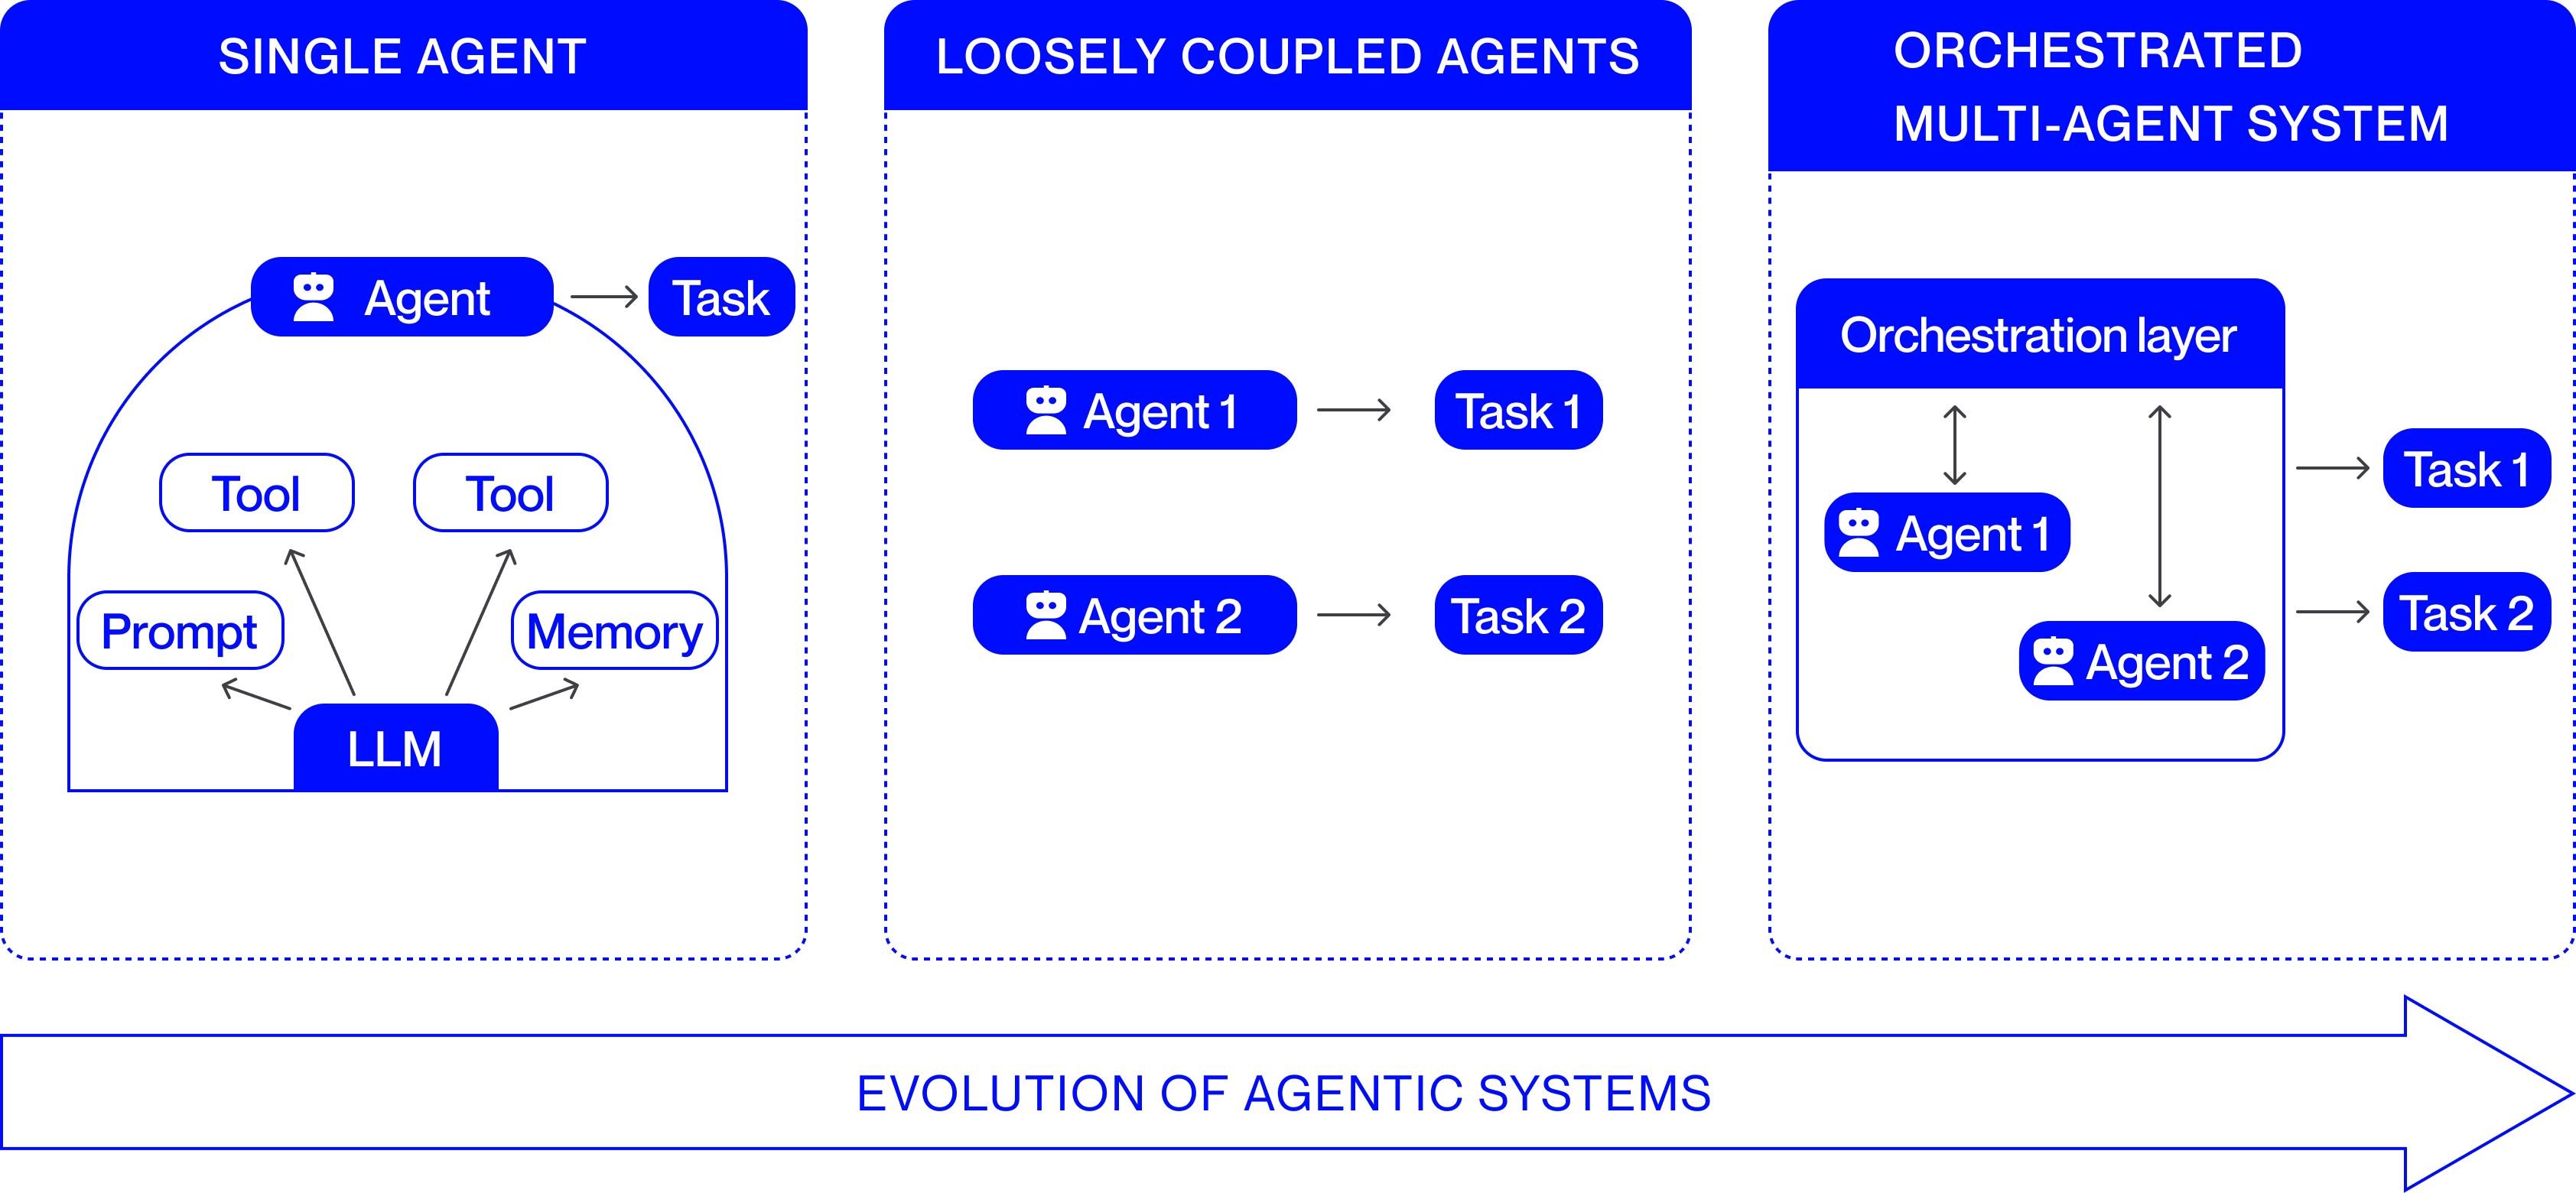
\includegraphics[width=\textwidth]{Images/chapter1/EvolutionAgenticSystems.png}
    \caption{Evolution of agentic system architectures: from a single LLM agent,
    to loosely coupled independent agents, to a fully orchestrated multi-agent system.
    Source:~\cite{agentsurvey2025}.}
    \label{fig:agent_evolution}
\end{figure}

\paragraph{Model Context Protocol.}
The \textbf{Model Context Protocol (MCP)}, introduced by Anthropic in
2024~\cite{anthropic2024mcp}, defines a standardized client-server protocol over a
\texttt{stdio} interface: tool servers expose a uniform schema describing their
capabilities, and agents discover and invoke tools dynamically at runtime. Each MCP
server encapsulates its own tools as independent, swappable modules
(Figure~\ref{fig:mcp_comparison}). In this project, MCP serves as the communication
backbone between Agent~2's ReAct loop and its web-research tool servers, enabling
search, scraping, and encyclopedic lookup through a uniform interface without any
tool-specific integration code in the agent itself.

\begin{figure}[H]
    \centering
    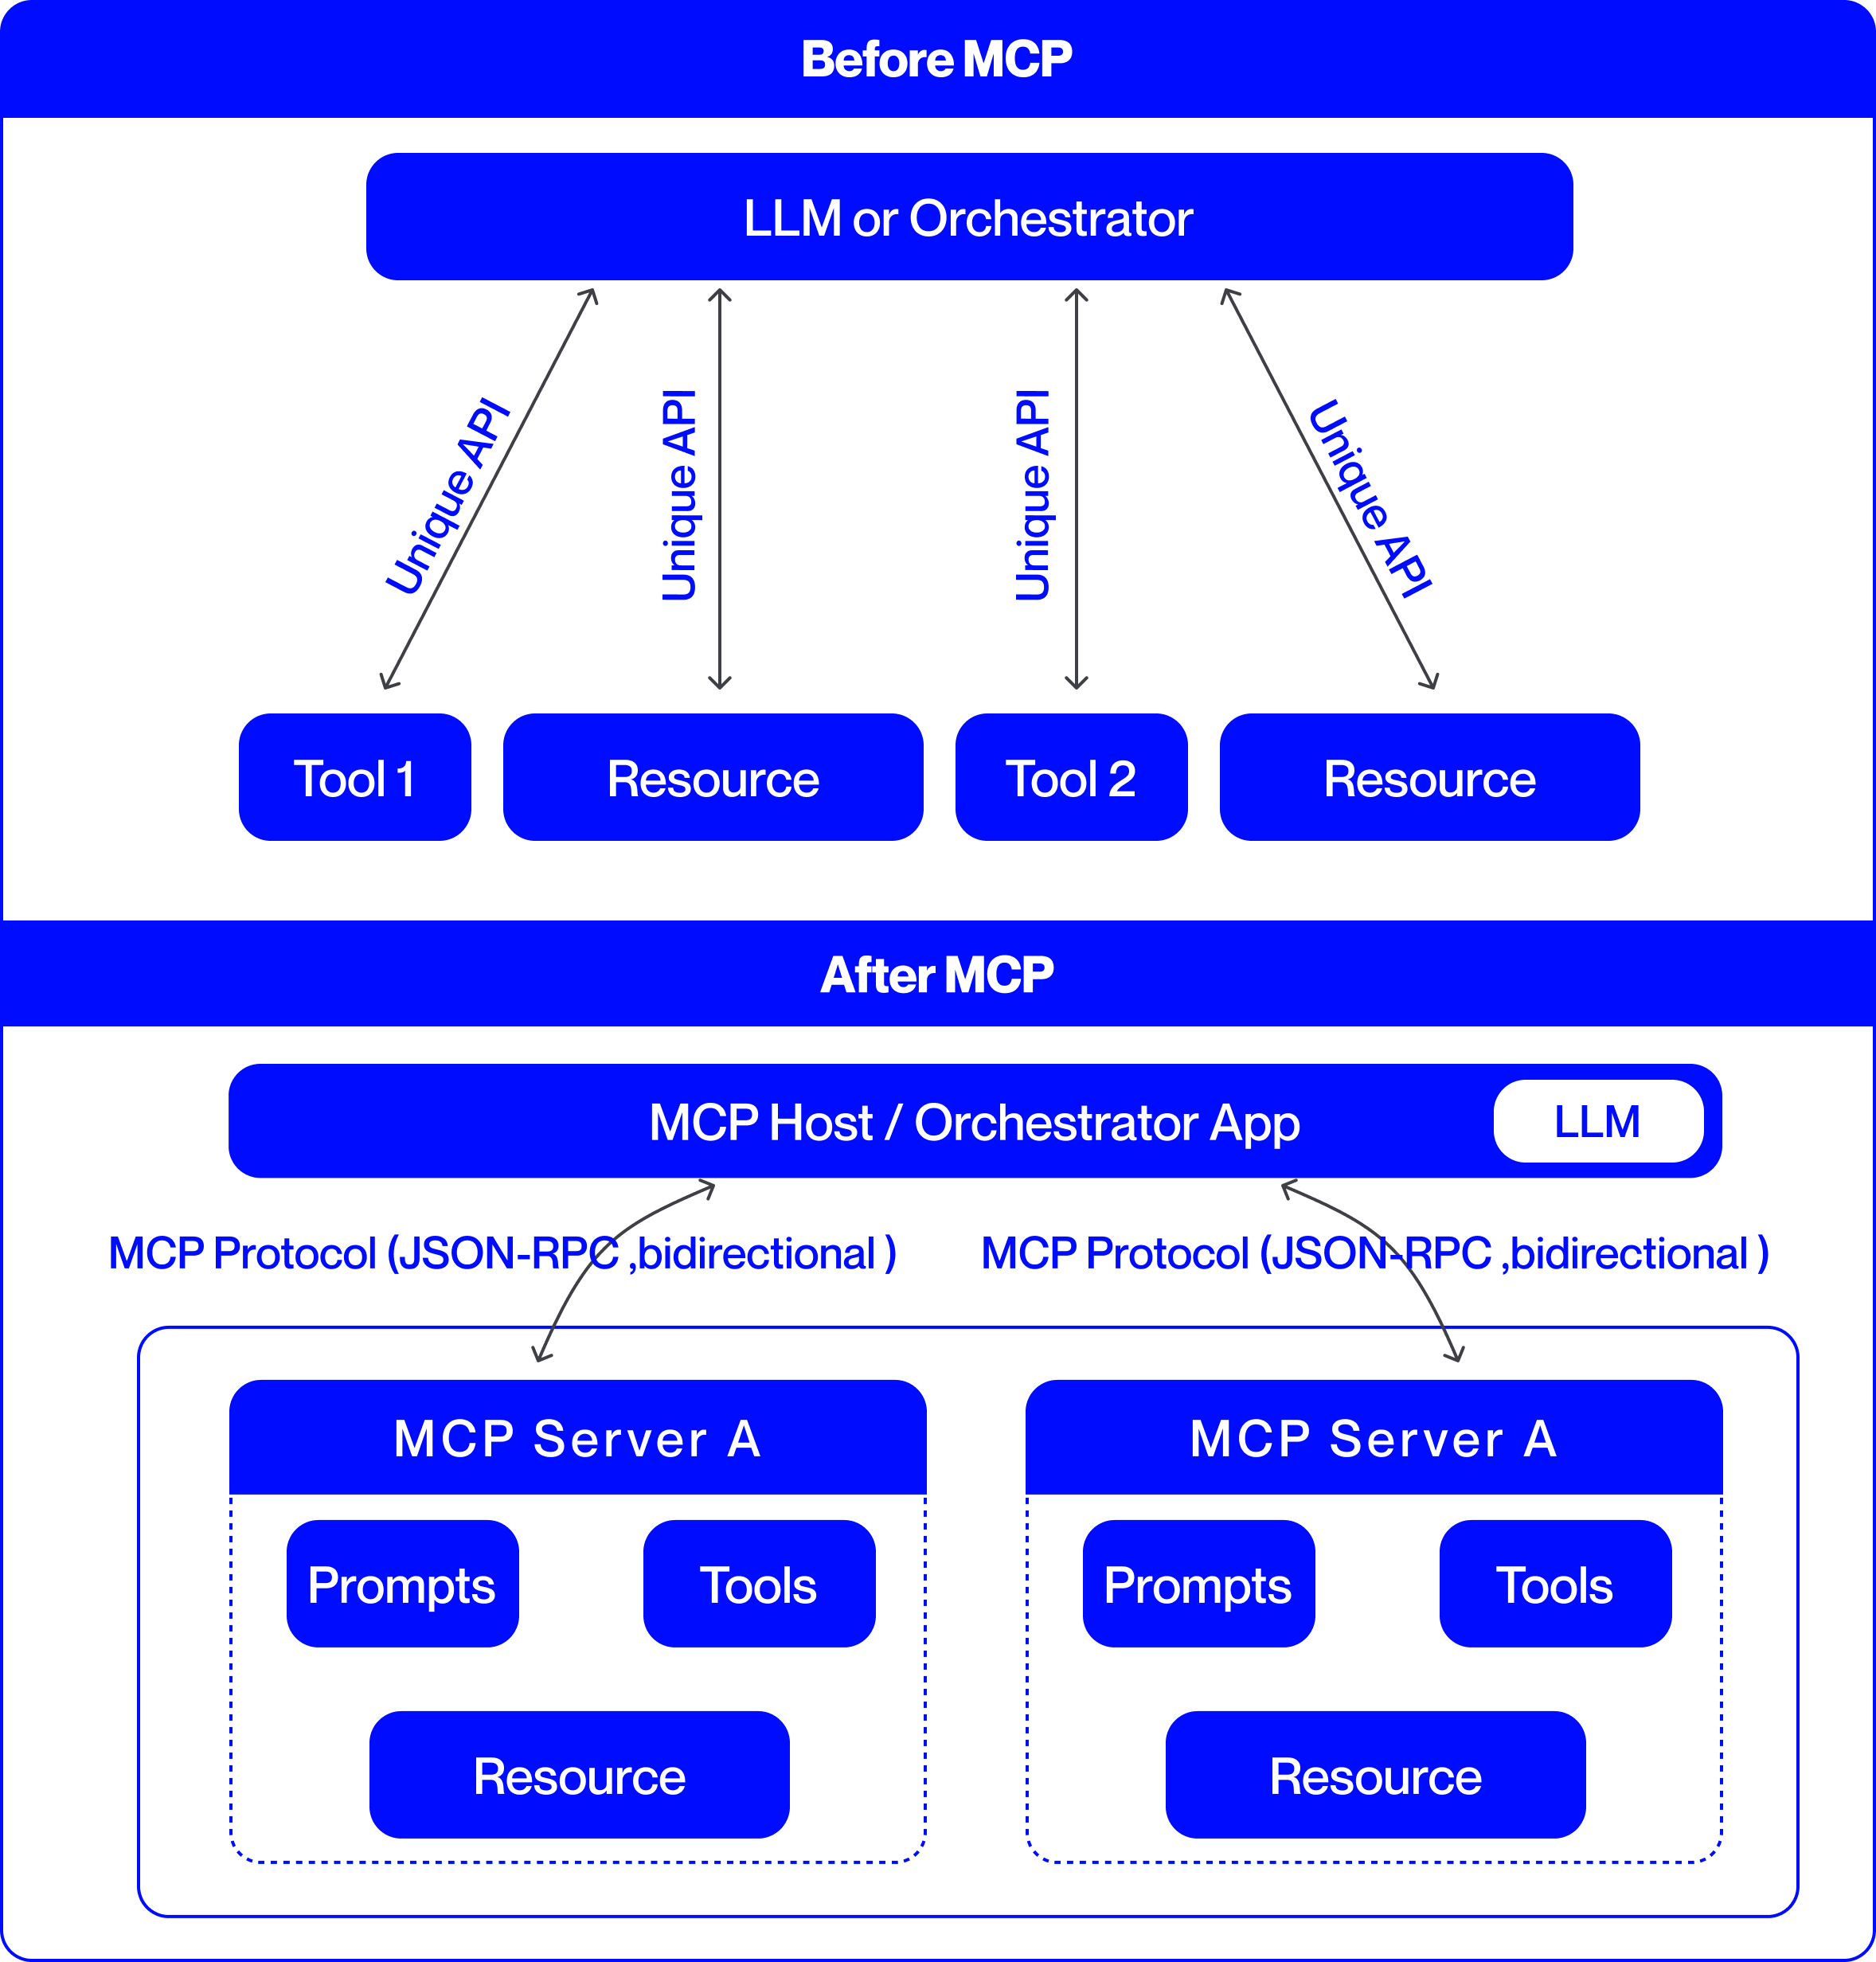
\includegraphics[width=0.7\textwidth]{Images/chapter1/BeforeVSAfter_v3.png}
    \caption{System architectures without and with MCP. Without MCP, the application
    must directly integrate each external tool. With MCP, a unified protocol layer
    mediates all interactions. Source:~\cite{agentsurvey2025}.}
    \label{fig:mcp_comparison}
\end{figure}

% ─────────────────────────────────────────────
\subsection{Related Work and Research Gaps}
\label{sec:related_work}

Despite growing interest in LLM-based visibility, no existing framework provides an
integrated, automated, and scientifically grounded solution for entity-level GEO
measurement.

\paragraph{Visual workflow automation tools.}
Platforms such as n8n~\cite{n8n2024} and Zapier support basic prompt submission and
response logging through predefined execution graphs, but offer no adaptive
decision-making, dynamic model selection, or cross-run statistical aggregation —
making them unsuitable for research-grade measurement.

\paragraph{Commercial GEO and AI visibility platforms.}
Tools including BrandGPT, Otterly.ai, and Profound monitor brand mentions in LLM
responses but with limited scientific validity: none discloses its measurement
methodology, they query a small fixed model set, and they do not support multi-run
evaluation essential for estimating mention stability~\cite{aggarwal2023geo}.

\paragraph{Summary of gaps.}
Table~\ref{tab:gaps} positions the contributions of this project against the key
limitations of existing approaches.

\begin{table}[H]
\centering
\caption{Limitations of existing approaches and contributions of the proposed system.}
\label{tab:gaps}
\begin{tabular}{|p{3.0cm}|p{4.6cm}|p{4.6cm}|}
\hline
\textbf{Aspect} & \textbf{Existing Approaches} & \textbf{This Project} \\
\hline
GEO measurement &
Manual or single-run, no cross-model analysis &
Automated, multi-prompt, multi-run, multi-model \\
\hline
Agent architecture &
Fixed execution graphs or visual workflows &
Autonomous ReAct orchestrator with runtime decision-making \\
\hline
Web data extraction &
Single source or manual lookup &
Multi-source extraction via MCP-based tool servers \\
\hline
Target domain &
Large, English-language brands &
Local entities in emerging and non-English markets \\
\hline
Statistical rigor &
Single-run, no stability analysis &
Mention rate, stability score, prominence index \\
\hline
\end{tabular}
\end{table}

Three gaps are of particular significance: no existing tool measures entity
visibility with statistical rigor across multiple prompts, runs, and models
simultaneously; no open framework automates the full pipeline from prompt generation
to web data extraction within a single autonomous system; and the relationship
between structured web presence signals and LLM visibility remains empirically
uninvestigated for local businesses in non-English markets. This project addresses
all three within a single integrated pipeline.

% ─────────────────────────────────────────────
\section*{Conclusion}
\addcontentsline{toc}{section}{\textbf{Conclusion}}

This chapter has traced the progression from link-based visibility governed by
documented algorithmic signals to representation-based visibility, where presence in
LLM-generated responses is an emergent property of training data coverage. As LLM
adoption scales globally, the asymmetry between well-represented global brands and
structurally neglected local businesses intensifies, making rigorous measurement
tools increasingly urgent. Existing approaches — visual automation platforms,
commercial monitoring dashboards, and single-model GEO tools — address this problem
only partially, each falling short in adaptability, rigor, or scope. These
limitations directly motivate the design of the system presented in the following
chapter.

%------------------------------------------chapter3  
\selectlanguage{english}
\chapter{System Design, Architecture, and Results}
\label{chap:design}
\renewcommand{\chaptername}{Chapter}

\section*{Introduction}
\addcontentsline{toc}{section}{\textbf{Introduction}}

This chapter presents the design, architecture, and preliminary results of the
proposed GEO measurement pipeline. It establishes the research approach and core
design decisions, then describes each component in detail: the dynamic model
registry, and the four specialized agents with their internal workflows. The chapter
concludes with preliminary evaluation results and a discussion of observed
limitations.

% ─────────────────────────────────────────────────────────────────────────────
\section{Research Approach and Design Philosophy}
% ─────────────────────────────────────────────────────────────────────────────

This project follows a \textbf{design science research} methodology
\cite{hevner2004design}: the primary contribution is a working software artifact
evaluated against the problem it was designed to solve. The approach involves
iterative construction and empirical evaluation --- each component is built, tested
under real API conditions, measured for output quality, and refined before the next
is designed. Three principles guided all architectural decisions.

\textbf{Autonomy over prescription:} the system makes its own decisions about which
model to use, which data source to query, and how to recover from failures ---
without human intervention at runtime. This ruled out fixed execution graphs in
favor of an orchestrator that reasons about the current state and selects the next
action dynamically.

\textbf{Resilience over speed:} the pipeline operates under constrained conditions
--- free-tier API quotas, variable rate limits, and tool servers that may time out.
The system must checkpoint progress and resume without data loss, motivating the
per-model state tracking in the model registry.

\textbf{Reproducibility over convenience:} all outputs are saved in structured CSV
files with fixed schemas. Intermediate outputs from each agent are preserved
separately so any stage can be re-run without repeating earlier stages.

% ─────────────────────────────────────────────────────────────────────────────
\section{System Overview}
% ─────────────────────────────────────────────────────────────────────────────

The pipeline is organized into four sequential stages, each handled by a dedicated
agent, coordinated by an orchestration layer, and supported by a dynamic model
registry shared across all agents. Figure~\ref{fig:system_overview} presents the
full system architecture.

\begin{figure}[H]
\centering
\begin{tikzpicture}[
  agent/.style={
    rectangle, rounded corners=5pt,
    draw=blue!65, fill=blue!8,
    text width=3.4cm, align=center,
    font=\small\bfseries, minimum height=1.0cm},
  orch/.style={
    rectangle, rounded corners=6pt,
    draw=violet!70, fill=violet!8,
    text width=2.4cm, align=center,
    font=\small\bfseries, minimum height=1.0cm},
  csv/.style={
    rectangle, rounded corners=3pt,
    draw=gray!55, fill=gray!5,
    text width=3.4cm, align=center,
    font=\scriptsize\itshape, minimum height=0.85cm},
  registry/.style={
    rectangle, rounded corners=5pt,
    draw=orange!70, fill=orange!8,
    text width=3.2cm, align=center,
    font=\small\bfseries, minimum height=0.9cm},
  provider/.style={
    rectangle, rounded corners=3pt,
    draw=red!40, fill=red!5,
    text width=2.8cm, align=center,
    font=\scriptsize, minimum height=0.6cm},
  mcp/.style={
    rectangle, rounded corners=3pt,
    draw=teal!60, fill=teal!7,
    text width=3.0cm, align=center,
    font=\scriptsize, minimum height=0.6cm},
  %% Arrow styles
  arrow/.style={-{Stealth[length=5pt]}, thick},
  darrow/.style={-{Stealth[length=4pt]}, thick, dashed, gray!60},
  oarrow/.style={-{Stealth[length=4pt]}, thick, orange!70},
  tarrow/.style={-{Stealth[length=4pt]}, thick, teal!65},
  earrow/.style={-{Stealth[length=4pt]}, thick, violet!65},
]

%% ═══════════════════════════════════════════════════════════════════════════
%% COLUMN POSITIONS
%%   Orchestrator  : x = -4.5   (left coordinator column)
%%   Agent column  : x =  0      (span: -1.7 to +1.7)
%%   CSV column    : x =  5.5    (span:  3.8 to  7.2)
%%   Routing lane  : x =  3.0    (gap between agent.east=1.7 and csv.west=3.8)
%%   Right column  : x =  9.8    (registry, providers, MCP)
%% ROW POSITIONS: y = 0, -3.5, -7.0, -10.5
%% ═══════════════════════════════════════════════════════════════════════════

%% ── Orchestrator (left column, vertically centered) ─────────────────────────
\node[orch] (orch) at (-4.5, -5.25) {Orchestrator\\{\footnotesize\normalfont orchestrator.py}};

%% ── Agents ──────────────────────────────────────────────────────────────────
\node[agent] (a0) at (0,    0)    {Agent 0\\{\footnotesize\normalfont Intent \& Prompts}};
\node[agent] (a1) at (0,   -3.5) {Agent 1\\{\footnotesize\normalfont Query \& Extract}};
\node[agent] (a2) at (0,   -7.0) {Agent 2\\{\footnotesize\normalfont Web Research}};
\node[agent] (a3) at (0,  -10.5) {Agent 3\\{\footnotesize\normalfont Merge \& Score}};

%% ── CSV checkpoints ─────────────────────────────────────────────────────────
\node[csv] (c0) at (5.5,    0)   {\texttt{prompt\_set.csv}\\{\tiny intents, prompts, language}};
\node[csv] (c1) at (5.5,  -3.5) {\texttt{entity\_features\_global.csv}\\{\tiny entities, mention\_rate, stability}};
\node[csv] (c2) at (5.5,  -7.0) {\texttt{web\_features.csv}\\{\tiny ratings, social, wikipedia}};
\node[csv] (c3) at (5.5, -10.5) {\texttt{enriched\_entities.csv}\\{\tiny all features + geo\_score}};

%% ── Model Registry + Providers (right column, rows 0–1 area) ────────────────
\node[registry] (reg)  at (9.8, -1.0)  {Dynamic Model\\Registry};
\node[provider] (groq) at (9.8, -2.5)  {Groq API};
\node[provider] (or)   at (9.8, -3.6)  {OpenRouter};
\node[provider] (mist) at (9.8, -4.7)  {Mistral API};

%% ── MCP Tool Servers (right column, row 2 area) ─────────────────────────────
\node[mcp] (mcp1) at (9.8, -6.2)  {Search Server\\{\tiny Maps · TA · DDG}};
\node[mcp] (mcp2) at (9.8, -7.2)  {Scrape Server\\{\tiny Instagram · Apify}};
\node[mcp] (mcp3) at (9.8, -8.2)  {Wiki Server\\{\tiny Wikipedia EN/FR}};

%% ═══════════════════════════════════════════════════════════════════════════
%% ARROWS
%% ═══════════════════════════════════════════════════════════════════════════

%% 0. Orchestrator → Agents  (sequential calls — fixed pipeline order)
%%    Route: orch.east → horizontal to x=-2.1, then bend down/up to each agent.west
\draw[earrow] (orch.east) -| (a0.west)
  node[near end, left, font=\scriptsize, violet!70] {(1)};
\draw[earrow] (orch.east) -| (a1.west)
  node[near end, left, font=\scriptsize, violet!70] {(2)};
\draw[earrow] (orch.east) -| (a2.west)
  node[near end, left, font=\scriptsize, violet!70] {(3)};
\draw[earrow] (orch.east) -| (a3.west)
  node[near end, left, font=\scriptsize, violet!70] {(4)};

%% 1. Agent → CSV  (horizontal writes, same row — always clear)
\draw[arrow] (a0.east) -- (c0.west)
  node[midway, above, font=\scriptsize] {writes};
\draw[arrow] (a1.east) -- (c1.west)
  node[midway, above, font=\scriptsize] {writes};
\draw[arrow] (a2.east) -- (c2.west)
  node[midway, above, font=\scriptsize] {writes};
\draw[arrow] (a3.east) -- (c3.west)
  node[midway, above, font=\scriptsize] {writes};

%% 2. CSV → next Agent  (sequential data feeds)
%%    Route: csv.south ↓ into the inter-row gap → left → agent.east
%%    All horizontals sit in clear inter-row gaps (no nodes there)

%% c0 → a1  (gap at y ≈ -1.75)
\draw[darrow]
  (c0.south) -- ++(0,-1.3) -| (a1.east)
  node[near start, right, font=\scriptsize, gray!70] {reads};

%% c1 → a2  (gap at y ≈ -5.25)
\draw[darrow]
  (c1.south) -- ++(0,-1.3) -| (a2.east);

%% c2 → a3  (gap at y ≈ -8.75)
\draw[darrow]
  (c2.south) -- ++(0,-1.3) -| (a3.east);

%% 3. c1 → a3  (Agent 3 also reads Agent 1 output — bypass via routing lane)
%%    Routing lane at x=3.0: between agent.east (1.7) and csv.west (3.8) — no nodes
\draw[darrow, gray!45]
  (c1.west)
    -- (3.0, -3.5)   %% enter the routing lane at row-1 level
    -- (3.0, -10.5)  %% descend to row-3 level (no nodes at x=3.0)
    -- (a3.east)
  node[near start, left, font=\scriptsize, gray!55] {also reads};

%% 4. Registry → LLM Providers  (downward within right column — always clear)
\draw[oarrow] (reg.south)  -- (groq.north);
\draw[oarrow] (groq.south) -- (or.north);
\draw[oarrow] (or.south)   -- (mist.north);

%% 5. Registry → Agent 1 and Agent 2  (model selection)
%%    Route: reg.west → routing lane (x=3.0) → agent.east
%%    Horizontal leg stays in the inter-row gap; vertical leg in clear lane

%% reg → a1: horizontal at y=-1.0 (between row-0 and row-1, no csv nodes there)
\draw[oarrow]
  (reg.west)
    -- (3.1, -1.0)   %% reach the routing lane at a clear y level
    -- (3.1, -3.5)   %% descend to row-1 in the lane
    -- (a1.east)
  node[near end, above, font=\scriptsize, orange!80] {model};

%% reg → a2: horizontal at y=-1.0 same entry, continues down to row-2
\draw[oarrow]
  (reg.west)
    -- (2.9, -1.0)   %% slightly offset to avoid exact overlap with reg→a1
    -- (2.9, -7.0)   %% descend to row-2 in the lane
    -- (a2.east);

%% 6. Agent 2 ↔ MCP Tool Servers
%%    Route: a2.east → ++(1.5,0) — reaching x=1.7+1.5=3.2 (in the lane)
%%    then right to MCP, staying above csv.south and below next row
\draw[tarrow]
  (a2.east) -- ++(2.0,0) |- (mcp1.west)
  node[near start, above, font=\scriptsize, teal!70] {tool calls};
\draw[tarrow] (a2.east) -- ++(2.0,0) |- (mcp2.west);
\draw[tarrow] (a2.east) -- ++(2.0,0) |- (mcp3.west);

%% ── Grouping boxes ──────────────────────────────────────────────────────────
\node[draw=teal!40, dashed, rounded corners=5pt,
      fit=(mcp1)(mcp2)(mcp3), inner sep=4pt,
      label={[font=\scriptsize\itshape, teal!60]above:MCP Tool Servers}] {};

\node[draw=red!30, dashed, rounded corners=5pt,
      fit=(groq)(or)(mist), inner sep=4pt,
      label={[font=\scriptsize\itshape, red!40]above:LLM Providers}] {};

\end{tikzpicture}
\caption{GEO pipeline data flow. The orchestrator (\texttt{orchestrator.py})
drives the four agents in fixed sequential order (1)–(4). Each agent reads its
input from the upstream CSV checkpoint and writes its output to the next.
Agent~3 merges both Agent~1 and Agent~2 outputs using fuzzy entity matching,
then applies LLM-based deduplication and entity triage.
Agents~1 and~2 query the dynamic model registry for the best available
(model, provider, key) triple at each inference call. Agent~2 performs all
web data collection exclusively through the three MCP tool servers.}
\label{fig:system_overview}
\end{figure}

% ─────────────────────────────────────────────────────────────────────────────
\section{Dynamic Model Registry}
% ─────────────────────────────────────────────────────────────────────────────

Operating across multiple free-tier LLM providers requires managing heterogeneous
and frequently binding quota constraints. The \textbf{dynamic model registry}
maintains a continuously updated state for every available model slot and selects
the best available option autonomously at each inference call --- eliminating the
need for hardcoded fallback chains.

At pipeline startup, the registry queries the model listing APIs of Groq, OpenRouter,
and Mistral, constructing a pool of slots identified by
\texttt{provider:keyIndex/model\_id}. Each slot is assigned a capability tier
(Table~\ref{tab:model_tiers}) and maintains three runtime states: \textbf{TPD
exhaustion} (daily quota hit --- permanent, persisted to disk across restarts),
\textbf{TPM block} (per-minute rate limit --- temporary, cleared when the retry
window expires), and \textbf{learned token capacity} (set on 413 errors --- used to
pre-filter the model for oversized prompts, eliminating repeated failures without
manual configuration).

\begin{table}[H]
\centering
\caption{Model capability tiers used for selection ranking.}
\label{tab:model_tiers}
\begin{tabular}{|c|p{3.2cm}|p{8.3cm}|}
\hline
\textbf{Tier} & \textbf{Quality Level} & \textbf{Identifying Keywords} \\
\hline
0 & Highest   & 70b, 72b, 120b, llama-4, qwen3-32b, claude-3.5, deepseek-r1 \\
\hline
1 & Medium    & 32b, 27b, 14b, gemini-flash, mistral-small, claude-3-haiku \\
\hline
2 & Lightweight & 8b, 7b, 3b, instant, mini, nano \\
\hline
\end{tabular}
\end{table}

The \texttt{select(preferred, estimated\_tokens)} method ranks candidates by tier,
provider, and key index --- but the pool it operates on evolves autonomously at
runtime. Three state transitions shape it without human intervention:
\texttt{mark\_tpd\_exhausted()} permanently removes a slot when its daily quota is
hit (persisted across restarts), \texttt{mark\_tpm()} blocks a slot until its
rate-limit window expires, and \texttt{mark\_too\_large()} records a learned
token-capacity ceiling on 413 errors so oversized prompts skip that model
automatically. The pipeline thus always selects the best \textit{currently usable}
model for the prompt at hand --- \textbf{adaptive autonomous selection} driven
entirely by the system's own API observations. The error-classification logic that
triggers these transitions lives in the Supervisor Agent
(Section~\ref{sec:supervisor}), described next.

% ─────────────────────────────────────────────────────────────────────────────
\section{Pipeline Agents}
% ─────────────────────────────────────────────────────────────────────────────

\subsection{Agent 0: Intent Discovery and Prompt Generation}

A single query formulation such as ``best restaurants in Tunis'' would produce
results sensitive to the experimenter's specific phrasing. Agent~0 addresses this
by autonomously generating a diverse prompt set covering multiple user intents and
linguistic variants, ensuring that downstream visibility metrics reflect robust
entity representation across a broad query space.

The generation pipeline consists of three steps. \textbf{Step 1 --- Intent
discovery:} given a domain description and target language, an LLM identifies
the distinct query intents a real user might have (e.g.\ recommendation requests,
occasion-based searches, comparison queries, information lookup). The number of
intents is controlled by the \texttt{n\_intents} parameter; the result is a
validated JSON taxonomy stored in the pipeline state. \textbf{Step 2 --- Prompt
generation:} for each intent and each target language (French and Arabic in this study),
\texttt{n\_variants} distinct formulations are generated using varied vocabulary,
sentence structure, and specificity level, simulating natural multilingual user
variation. \textbf{Step 3 --- Self-reflection:} the LLM evaluates the \textit{entire} prompt
set against quality criteria: intent diversity, linguistic naturalness, and a
GEO-specific constraint requiring that at least 60\% of prompts force the AI to
name specific establishments (using superlatives, rankings, or explicit citation
requests). If the set fails (\texttt{proceed: false}), the whole generation is
restarted with the missing intents added to \texttt{n\_intents}; the loop runs at
most \texttt{max\_reflection\_loops} times (default~2). The final set is saved to
\texttt{prompt\_set.csv}.

\begin{figure}[H]
\centering
\begin{tikzpicture}[
  box/.style={rectangle, rounded corners=4pt, draw=blue!60, fill=blue!8,
              text width=3.8cm, align=center, font=\small, minimum height=1.0cm},
  decision/.style={rectangle, rounded corners=4pt, draw=orange!70, fill=orange!8,
                   text width=3.0cm, align=center, font=\scriptsize,
                   minimum height=0.8cm},
  arrow/.style={-{Stealth[length=5pt]}, thick},
  io/.style={rectangle, rounded corners=4pt, draw=green!60!black, fill=green!7,
             text width=3.4cm, align=center, font=\small, minimum height=0.8cm},
]
\node[io]       (input)   at (0, 0)    {Domain + Language\\+ Parameters};
\node[box]      (intents) at (0, -2.0) {Step 1 --- Intent Discovery\\{\footnotesize LLM intent taxonomy}};
\node[box]      (prompts) at (0, -4.0) {Step 2 --- Prompt Generation\\{\footnotesize n\_variants per intent}};
\node[box]      (reflect) at (0, -6.0) {Step 3 --- Self-Reflection\\{\footnotesize quality scoring}};
\node[decision] (check)   at (0, -8.0) {All prompts pass\\quality threshold?};
\node[io]       (output)  at (5.5, -8.0) {\texttt{prompt\_set.csv}};
\draw[arrow] (input)   -- (intents);
\draw[arrow] (intents) -- (prompts);
\draw[arrow] (prompts) -- (reflect);
\draw[arrow] (reflect) -- (check);
\draw[arrow] (check.east) -- (output.west)
  node[midway, above, font=\scriptsize] {Yes};
\draw[arrow] (check.west) -- ++(-2.5, 0) |- (prompts.west)
  node[near start, left, font=\scriptsize, align=center] {No\\regenerate};
\end{tikzpicture}
\caption{Agent~0 workflow: intent discovery, prompt generation, and self-reflection
quality control. Low-quality prompts trigger a targeted regeneration loop.}
\label{fig:agent0_flow}
\end{figure}

\subsection{Agent 1: LLM Querying and Entity Extraction}

Agent~1 is responsible for the core GEO measurement task: submitting the generated
prompts to multiple LLMs across independent runs, extracting the named entities
mentioned in each response, and computing visibility metrics that quantify how
consistently each entity appears across the full prompt, model, and run space.

\textbf{Step 2 --- Multi-model querying.} Each prompt is submitted to every
model slot in the \texttt{QUERY\_MODELS} configuration, repeated \texttt{n\_runs}
times per slot. This cross-model, multi-run design is the core of GEO measurement:
entity visibility is only meaningful when aggregated across diverse LLMs and
phrasing variants, not a single model call. All responses are appended
progressively to \texttt{raw\_responses.csv} with resume support.

\textbf{Step 3 --- Zero-shot entity extraction.} A dedicated Mistral extractor
(fixed model, temperature~0) processes each raw response with a detailed system
prompt specifying domain scope (Tunisian establishments only), normalization rules
(lowercase, strip generic prefixes), and output format (flat JSON string array).
The extractor returns entity names only --- no confidence scores --- along with the
text block describing each entity for downstream context.

\textbf{Step 4 --- Enrichment.} For each extracted entity, two structural features
are computed: \textbf{ranking position} (the order in which the entity first
appeared in the response, extracted via a second LLM call over the ranked list) and
\textbf{description length in tokens} (estimated from the character ratio of the
entity's description block to the full response).

\textbf{Step 5 --- Five-phase cleaning pipeline.}
(A)~\textbf{Hard pre-filtering} drops empty, too-short ($<$3 chars), numeric, and
singleton entries (mention count $<$ 2) --- singletons are noise, not signal.
(B)~\textbf{Fuzzy clustering} (RapidFuzz, threshold~88) groups high-similarity
names; the most frequent variant in each cluster becomes the canonical form.
(C)~\textbf{LLM arbitration} resolves ambiguous pairs (similarity 75--87) and
simultaneously validates every entity: entities that are generic descriptors, wrong
geography, or lack Tunisian context are invalidated.
(D)~\textbf{Self-reflection} reviews all cleaning decisions and immediately applies
corrections --- undoing incorrect merges or invalidations flagged as suspicious.
(E)~\textbf{Mapping application} writes the final canonical names, quality flags,
and null-rank penalties to \texttt{clean\_entities.csv}.

\textbf{Step 6 --- GEO metric computation.} Three visibility metrics are computed
per canonical entity across all responses: \textbf{mention rate} (fraction of
valid responses in which the entity appeared), \textbf{stability score}
($\text{mention\_rate} \times \frac{1}{1+\text{rank\_variance}}$, combining
frequency with positional consistency), and a \textbf{consistency label}
(\textit{stable} $\geq$~0.75, \textit{variable} $\geq$~0.40, \textit{unstable}
otherwise). Entities with fewer than 2 mentions are excluded at Phase~A; the
stability threshold for Agent~2 eligibility is applied by the orchestrator.

\begin{figure}[H]
\centering
\begin{tikzpicture}[
  box/.style={rectangle, rounded corners=4pt, draw=blue!60, fill=blue!8,
              text width=4.0cm, align=center, font=\small, minimum height=1.0cm},
  arrow/.style={-{Stealth[length=5pt]}, thick},
  io/.style={rectangle, rounded corners=4pt, draw=green!60!black, fill=green!7,
             text width=3.4cm, align=center, font=\small, minimum height=0.8cm},
]
\node[io]  (input)   at (0, 0)     {\texttt{prompt\_set.csv}};
\node[box] (query)   at (0, -2.0)  {Step 2 --- Multi-model Querying\\{\footnotesize QUERY\_MODELS $\times$ n\_runs}};
\node[box] (extract) at (0, -4.0)  {Step 3 --- Entity Extraction\\{\footnotesize Mistral, flat JSON, names only}};
\node[box] (enrich)  at (0, -6.0)  {Step 4 --- Enrichment\\{\footnotesize ranking position + desc.\ length}};
\node[box] (clean)   at (0, -8.0)  {Step 5 --- Cleaning (A--E)\\{\footnotesize hard rules · fuzzy · LLM · reflect}};
\node[box] (metrics) at (0, -10.0) {Step 6 --- GEO Metrics\\{\footnotesize mention rate, stability score}};
\node[io]  (output)  at (0, -12.0) {\texttt{entity\_features\_global.csv}};
\draw[arrow] (input)   -- (query);
\draw[arrow] (query)   -- (extract)
  node[midway, right, font=\scriptsize] {\texttt{raw\_responses.csv}};
\draw[arrow] (extract) -- (enrich)
  node[midway, right, font=\scriptsize] {\texttt{extracted\_entities.csv}};
\draw[arrow] (enrich)  -- (clean)
  node[midway, right, font=\scriptsize] {\texttt{enriched\_entities.csv}};
\draw[arrow] (clean)   -- (metrics)
  node[midway, right, font=\scriptsize] {\texttt{clean\_entities.csv}};
\draw[arrow] (metrics) -- (output);
\end{tikzpicture}
\caption{Agent~1 workflow: multi-model querying, entity extraction, enrichment,
five-phase cleaning, and GEO metric computation. Each intermediate output is
checkpointed to CSV for resume support.}
\label{fig:agent1_flow}
\end{figure}

\subsection{Agent 2: Web Presence Research}

Agent~2 is the most technically complex component. For each entity meeting the
visibility threshold, it operates as a fully autonomous ReAct agent over three
MCP tool servers --- at each step it produces a \textit{thought} about what
information has been gathered so far, selects a \textit{tool invocation} as its
\textit{action}, and incorporates the tool's response as an \textit{observation}
before deciding the next step.

The agent follows a \textbf{prescribed 8-step research protocol} defined in its
system prompt: (1)~\texttt{google\_maps\_search}, (2)~\texttt{wikipedia\_lookup},
(3)~\texttt{tripadvisor\_search}, (4)~\texttt{wikidata\_lookup}, then conditionally:
(5)~\texttt{extract\_website\_socials} if a website was found, (6)~\texttt{scrape\_instagram}
if an Instagram handle was found, (7)~\texttt{scrape\_facebook} if a Facebook handle
was found, and (8)~\texttt{ddg\_search} if no social presence was located. Steps 1--4
always execute in order; steps 5--8 depend on what earlier steps returned.
The ReAct loop provides adaptive handling of tool failures and observations, but the
sequence of data targets is fixed.

The four MCP servers expose the tools described in Table~\ref{tab:mcp_tools}. The
protocol collects data across six categories (Google Maps, TripAdvisor, Wikipedia,
Wikidata, Instagram, Facebook) and enforces geographic anchoring: every search query
must include ``Tunisia'' or a Tunisian city name, and any result referencing a
non-Tunisian geographic context is discarded and the search retried with more
specific terms.

\begin{table}[H]
\centering
\caption{MCP tool servers and their exposed tools.}
\label{tab:mcp_tools}
\begin{tabular}{|p{2.5cm}|p{3.5cm}|p{7.2cm}|}
\hline
\textbf{Server} & \textbf{Tool} & \textbf{Description} \\
\hline
\multirow{3}{*}{search\_server}
  & \texttt{google\_maps\_search}      & Rating, review count, address, phone, website. Rotates through a pool of SerpAPI keys. \\
\cline{2-3}
  & \texttt{tripadvisor\_search}       & Two-step: web search locates the TA page URL, then scraper extracts rating and ranking. \\
\cline{2-3}
  & \texttt{ddg\_search}               & General DuckDuckGo search returning titles, URLs, snippets. \\
\hline
\multirow{3}{*}{scrape\_server}
  & \texttt{scrape\_instagram}         & Follower count, post count, biography via Apify. Rotates through 5 Apify tokens. \\
\cline{2-3}
  & \texttt{scrape\_facebook}          & Page likes and average post engagement via Apify. \\
\cline{2-3}
  & \texttt{extract\_website\_socials} & Extracts Instagram/Facebook handles from a business website's HTML. \\
\hline
wiki\_server
  & \texttt{wikipedia\_lookup}         & Queries the Wikipedia API in English and French; returns boolean presence and URL. \\
\hline
enrichment\_server
  & \texttt{wikidata\_lookup}          & Queries the Wikidata API; returns entity type, country, founded date, and official website. \\
\hline
\end{tabular}
\end{table}

\subsubsection*{Supervisor Agent}
\label{sec:supervisor}

API errors are handled by the \textbf{Supervisor Agent} --- a rule-based error
classifier with an optional LLM escalation path --- that inspects each error message
and returns a structured recovery decision
with four possible actions: \texttt{switch\_model} (billing or quota exhaustion ---
mark slot TPD-exhausted), \texttt{wait\_retry} (rate limit --- wait the extracted
retry-after duration), \texttt{retry} (transient 5xx --- retry immediately), or
\texttt{skip} (unrecoverable after 4 attempts). Internally, the supervisor first
attempts to call a lightweight LLM on the error text; if that call fails or times
out, it falls back to a deterministic \texttt{if/elif} chain that encodes the same
classification rules explicitly. In practice the LLM and the fallback produce
identical decisions for the structured error codes that providers return --- the LLM
path adds resilience for novel or ambiguous error messages, not a fundamentally
different decision process. Each successfully processed entity is immediately
checkpointed to \texttt{web\_features.csv}.

\begin{figure}[H]
\centering
\begin{tikzpicture}[
  box/.style={rectangle, rounded corners=4pt, draw=blue!60, fill=blue!8,
              text width=3.6cm, align=center, font=\small, minimum height=1.0cm},
  supervisor/.style={rectangle, rounded corners=4pt, draw=red!50, fill=red!6,
              text width=3.2cm, align=center, font=\small, minimum height=1.0cm},
  mcp/.style={rectangle, rounded corners=4pt, draw=teal!60, fill=teal!7,
              text width=3.2cm, align=center, font=\small, minimum height=1.0cm},
  io/.style={rectangle, rounded corners=4pt, draw=green!60!black, fill=green!7,
             text width=3.2cm, align=center, font=\small, minimum height=0.8cm},
  arrow/.style={-{Stealth[length=5pt]}, thick},
]
\node[io]         (input)  at (0, 0)     {Entity Name + Context};
\node[box]        (think)  at (0, -2.0)  {Thought\\Reason about gathered data};
\node[box]        (act)    at (0, -4.0)  {Action\\Select \& invoke MCP tool};
\node[mcp]        (mcp)    at (5.0, -4.0){MCP Tool Servers\\Search · Scrape · Wiki · Enrichment};
\node[box]        (obs)    at (0, -6.0)  {Observation\\Parse \& validate result};
\node[box]        (check)  at (0, -8.0)  {Sufficient data\\collected?};
\node[supervisor] (sup)    at (5.0, -6.5){Supervisor Agent\\Classify error\\Return action};
\node[io]         (output) at (0, -10.5) {\texttt{web\_features.csv}};
\draw[arrow] (input)  -- (think);
\draw[arrow] (think)  -- (act);
\draw[arrow] (act.east)  -- (mcp.west)  node[midway, above, font=\scriptsize] {tool call};
\draw[arrow] (mcp.west)  -- (obs.east)  node[midway, below, font=\scriptsize] {result};
\draw[arrow] (obs)    -- (check);
\draw[arrow] (check.west) -- ++(-2.2, 0) |- (think.west)
  node[near start, left, font=\scriptsize, align=center] {No\\next step};
\draw[arrow] (check.south) -- (output)  node[midway, right, font=\scriptsize] {Yes};
\draw[arrow, red!50, dashed] (obs.east)  -- (sup.west)
  node[midway, above, font=\scriptsize] {on error};
\draw[arrow, red!50, dashed] (sup.north) -- ++(0, 0.6) -| (act.east)
  node[near start, right, font=\scriptsize, align=center] {retry /\\switch model};
\end{tikzpicture}
\caption{Agent~2 ReAct processing loop. The agent iterates
Thought--Action--Observation cycles over MCP tool servers until sufficient web
presence data has been collected. All errors are handled by the Supervisor Agent,
which reasons about the failure type and returns a structured recovery action
without terminating the loop.}
\label{fig:agent2_flow}
\end{figure}

\subsection{Agent 3: Merge, Deduplication, and Agentic Triage}

Agent~3 is the final stage of the pipeline. It joins the LLM visibility metrics
from Agent~1 with the web presence features from Agent~2 using a three-stage fuzzy
matching strategy (exact normalized match, substring containment, then word overlap),
with Agent~1 as the source of truth so that every extracted entity is retained.

Two LLM-based reasoning steps then clean the merged dataset. First,
\textbf{deduplication}: entities are grouped by shared content words (stop words
such as \textit{le, la, de, el, dar} removed) and each candidate group is submitted
to the LLM to decide whether the rows refer to the same place. Confirmed duplicates
are merged --- mention counts summed, the richer web-data row kept.
Second, \textbf{triage}: entities for which Agent~2 found no web evidence are
classified by the LLM as \textit{retry} (real restaurant, missed by Agent~2),
\textit{hallucination}, \textit{non\_restaurant}, or \textit{generic}.
Non-viable entities are removed and saved to \texttt{rejected\_entities.csv};
\textit{retry} entities are written to the merge report so the orchestrator can
re-invoke Agent~2 on them.

Finally, Agent~3 computes a \textbf{data-completeness score} (fraction of ten key
fields that are non-null) and assigns a \textbf{unified quality} label
(\textit{complete}, \textit{partial}, \textit{sparse}, or \textit{agent2\_failed})
to each row. The result is saved to \texttt{unified\_features.csv}.
Table~\ref{tab:output_schema} lists the key output fields.

\begin{table}[H]
\centering
\caption{Key fields in the final output dataset (\texttt{unified\_features.csv}).}
\label{tab:output_schema}
\begin{tabular}{|p{3.8cm}|p{2.2cm}|p{7.2cm}|}
\hline
\textbf{Field} & \textbf{Source} & \textbf{Description} \\
\hline
\texttt{canonical\_entity}   & Agent 1 & Normalized entity name \\
\texttt{mention\_rate}       & Agent 1 & Fraction of valid responses with a mention \\
\texttt{stability\_score}    & Agent 1 & $\text{mention\_rate} \times \frac{1}{1+\text{rank\_variance}}$ \\
\texttt{consistency\_label}  & Agent 1 & stable / variable / unstable \\
\texttt{gm\_rating}          & Agent 2 & Google Maps rating (0--5) \\
\texttt{gm\_review\_count}   & Agent 2 & Google Maps number of reviews \\
\texttt{ta\_rating}          & Agent 2 & TripAdvisor rating \\
\texttt{ta\_ranking}         & Agent 2 & TripAdvisor ranking position \\
\texttt{has\_wikipedia}      & Agent 2 & Boolean Wikipedia presence \\
\texttt{ig\_followers}       & Agent 2 & Instagram follower count \\
\texttt{overall\_confidence} & Agent 2 & Agent-assigned data quality score (0--1) \\
\texttt{data\_completeness}  & Agent 3 & Fraction of key fields non-null (0--1) \\
\texttt{unified\_quality}    & Agent 3 & complete / partial / sparse / agent2\_failed \\
\texttt{triage\_decision}    & Agent 3 & retry / hallucination / non\_restaurant / generic (failed entities only) \\
\texttt{triage\_reason}      & Agent 3 & LLM justification for the triage decision \\
\hline
\end{tabular}
\end{table}

% ─────────────────────────────────────────────────────────────────────────────
\section{Results}
% ─────────────────────────────────────────────────────────────────────────────

The pipeline was applied to the Tunisian restaurant domain. Agent~0 generated
\textbf{30 prompts} covering \textbf{6 distinct user intents} (top recommendation,
tourist reviews, comparative, authentic cuisine, special occasion, location-based)
with 5~variants each in French. Agent~1 submitted each prompt to
\textbf{3 model slots}, repeated 5~times per slot, yielding \textbf{450 total
responses}. From these, 2{,}020 raw entity extraction records (831 unique surface
forms) were produced, which the five-phase cleaning pipeline consolidated into
\textbf{234 canonical entities}.

Of the 234 entities, \textbf{213 met the eligibility threshold} (minimum mention
rate) and were submitted to Agent~2 for web enrichment. Agent~3 then applied
LLM-based deduplication to collapse variant spellings of the same establishment
(e.g., \textit{Dar El Jeld} vs.\ \textit{Dar el Jeld Restaurant}) and
LLM-based triage to remove non-viable entries: 4~entities were rejected
(1~hallucination, 1~non-restaurant venue, 2~over-generic names). The final
dataset contains \textbf{182 enriched entities}. Table~\ref{tab:pipeline_results}
summarizes the key metrics from the actual output files.

\begin{table}[H]
\centering
\caption{Pipeline results on the Tunisian restaurant domain.}
\label{tab:pipeline_results}
\begin{tabular}{|p{7cm}|r|}
\hline
\textbf{Metric} & \textbf{Value} \\
\hline
Prompts generated (Agent 0)                          & 30 \\
LLM responses collected (Agent 1)                    & 450 \\
Raw entity extraction records                        & 2{,}020 \\
Unique surface forms before cleaning                 & 831 \\
Canonical entities after cleaning                    & 234 \\
Entities submitted to Agent 2                        & 213 \\
Final entities after dedup + triage (Agent 3)        & 182 \\
\quad — Complete ($\geq$3 sources)                   & 75 \\
\quad — Partial (1--2 sources)                       & 84 \\
\quad — Failed (no sources recovered)                & 22 \\
Entities rejected by LLM triage                      & 4 \\
Google Maps coverage                                 & 85.2\% \\
TripAdvisor coverage                                 & 38.5\% \\
Wikipedia presence                                   & 0\% \\
Instagram presence                                   & 31.9\% \\
Facebook presence                                    & 28.0\% \\
Mean data-completeness score                         & 0.584 \\
Mean overall confidence score                        & 0.541 \\
\hline
\end{tabular}
\end{table}

The distribution of LLM visibility is strongly concentrated: the top 15\% of
entities (27 out of 182) accumulate 62\% of all 1{,}351 mention instances, while
the remaining 85\% share the other 38\%. The single most-visible establishment,
\textit{Dar El Jeld}, received 159 mentions across all prompts and model slots ---
more than twice the count of the second-ranked entity. All entities carry an
\textit{unstable} consistency label, which is expected given the limited prompt set
(30 prompts) and the high variance of mention rates at this scale. The zero
Wikipedia coverage confirms that none of the 182 entities has a dedicated Wikipedia
article, consistent with the local and informal character of the Tunisian restaurant
market. The moderate Instagram and Facebook presence (32\% and 28\% respectively)
reflects the partial digitalization of small hospitality businesses in Tunisia.

% ─────────────────────────────────────────────────────────────────────────────
\section{Limitations and Discussion}
% ─────────────────────────────────────────────────────────────────────────────

Despite the agentic design improvements, several limitations were encountered.

\textbf{Partial web enrichment.} Of the 182 final entities, 22 (12\%) remain in a
\textit{failed} state after one enrichment pass and a second targeted retry pass.
These are restaurants whose names are either too common (shared with many
unrelated venues), spelled inconsistently across sources, or genuinely absent from
indexed web pages. Improving recall for this tail would require more specific
search strategies, such as incorporating city-level geocoding into the SerpAPI
query or combining multiple web sources per entity.

\textbf{Geographic disambiguation.} A number of entity names extracted from LLM
responses refer to well-known establishments outside Tunisia --- for example,
\textit{Le Grand Véfour} (Paris) or \textit{La Mamounia} (Marrakech hotel) ---
that are far better represented in LLM training data than any Tunisian homonym.
Agent~3's LLM triage successfully identified and rejected 4 such non-viable
entities, but the root cause lies upstream: Agent~0 prompts should more
aggressively enforce geographic specificity to prevent the LLM from surfacing
non-Tunisian establishments in the first place.

\textbf{Social media data sparsity.} Only 31.9\% of the 182 entities carry an
identified Instagram handle and 28.0\% a Facebook page, reflecting the relatively
low digital formalization of small hospitality businesses in the Tunisian market.
This sparsity limits the social dimension of the GEO score for the majority of
entities, and may understate the actual social media presence of establishments
that operate under informal or unverified page names.

\textbf{Triage robustness and JSON fragility.} The LLM triage step in Agent~3
serializes entity names into JSON prompts. Entity names containing apostrophes
(e.g., \textit{la table d'or}) caused JSON parse failures in initial runs,
requiring a robust fallback parser (\texttt{\_parse\_json\_objects}) that extracts
individual JSON objects when the full array parse fails. This fragility is an
inherent risk of relying on LLM-generated structured output and should be
addressed by escaping entity names before injection or switching to a
tool-calling interface.

\textbf{Retry convergence.} The two-pass retry design (Agent~2 $\rightarrow$
Agent~3 triage $\rightarrow$ Agent~2 retry) leaves 21 entities in a pending retry
queue at the end of the observed execution. A fully converged pipeline would
require either a third pass or a dedicated loop termination criterion (e.g., no
improvement after two consecutive retries).

\textbf{API quota and rate-limit constraints.}
The pipeline relies on three categories of external APIs, each with distinct
failure modes. \textit{LLM inference APIs} (Groq, OpenRouter, Together AI, Mistral)
impose per-minute and per-day token quotas on free tiers; hitting these limits
mid-pipeline caused request timeouts and forced the dynamic model registry to
cycle through fallback models, sometimes exhausting all available slots before a
batch completed. \textit{SerpAPI}, used by Agent~2 for Google Maps and TripAdvisor
lookups, provides only 100 free queries per key; with 213 entities requiring
multiple search queries each, the five available keys were consumed in a single
execution pass, leaving a subset of entities without web data until the keys
reset. \textit{Wikidata and Instagram} imposed no hard quotas but required
progressive throttling (sleep intervals between requests) to avoid HTTP~429
responses. Collectively, these constraints forced pipeline execution to be split
across multiple sessions on different days, introducing a temporal inconsistency in
the collected data. A production deployment would require paid API tiers or
self-hosted inference to run the full pipeline in a single uninterrupted pass.

\subsection*{Toward a GEO-Based Recommendation System}

Beyond measurement, the ultimate objective of this project is to build a
\textbf{recommendation system for brand visibility in generative AI}.
The pipeline described in this chapter constitutes the data acquisition and
diagnostic layer: it quantifies, for each restaurant, how visible it currently is
to LLM-based search engines and how complete its digital footprint is across the
web. The next step is to exploit this dataset to generate \textit{actionable
recommendations} --- identifying, for each brand, the specific levers that would
increase its likelihood of being cited by an AI assistant.

Concretely, a low \texttt{mention\_rate} combined with high \texttt{gm\_review\_count}
suggests that the brand has real-world credibility but lacks the textual signal
(structured web mentions, linked data, editorial coverage) that LLMs rely on
during pre-training. Conversely, a brand with high LLM visibility but low
TripAdvisor coverage may benefit from consolidating its review presence to
reinforce consistency across sources. The GEO score synthesizes these dimensions
into a single prioritization signal, enabling the recommendation engine to rank
optimization actions by expected impact on generative visibility.

This framing --- measuring current AI visibility, diagnosing its root causes,
and prescribing targeted improvements --- positions the system as a practical
tool for restaurant owners and marketers who wish to compete in the emerging
landscape where AI-generated responses, rather than ranked search results, drive
consumer discovery.

% ─────────────────────────────────────────────────────────────────────────────
\section*{Conclusion}
\addcontentsline{toc}{section}{\textbf{Conclusion}}
% ─────────────────────────────────────────────────────────────────────────────

This chapter has presented the full design, architecture, and results of the GEO
measurement pipeline. The four agents --- each with a well-defined input, processing
workflow, and structured output --- collectively realize the three design principles:
autonomy through supervisor-based error recovery, registry-driven model selection,
and LLM-based deduplication and triage; resilience through progressive checkpointing,
fuzzy entity matching, and a two-pass retry loop; and reproducibility through fixed
CSV schemas and decoupled outputs. Applied to the Tunisian restaurant domain, the
pipeline produced a final enriched dataset of \textbf{182 entities} with 85.2\%
Google Maps coverage and a mean data-completeness of 0.584, confirming both a
strong concentration of LLM visibility (top 15\% of entities attract 62\% of
mentions) and the practical challenges of web data acquisition for local businesses.
These findings provide the analytical dataset from which the research questions
posed in Chapter~1 will be systematically investigated in the following chapters.

%------------------------------------------chapter4
\chapter{Implementation and Evaluation}
\label{chap:impl}

The preceding chapter defined the GEO pipeline at the architectural level.
This chapter documents how that architecture was translated into a working system:
the technology choices made under real resource constraints, the non-trivial
engineering decisions that the design left open, the concrete failures encountered
during development and how they were resolved, and the experimental results
obtained on the Tunisian restaurant domain.

% ═══════════════════════════════════════════════════════════════════════════════
\section{Development Environment and Technology Stack}
\label{sec:devenv}
% ═══════════════════════════════════════════════════════════════════════════════

The system was implemented in \textbf{Python 3.11} on a standard Windows 10 machine,
without access to dedicated GPU hardware. This constraint is not incidental: it reflects
the reality of academic research conducted outside industrial infrastructure, and it
directly shaped every technology choice made throughout the project.

Three design imperatives governed the selection of components.
The first was \textit{cost accessibility}: all LLM inference had to operate within
free or low-cost API tiers, since sustained experimentation across hundreds of queries
would otherwise be financially prohibitive. This requirement alone motivated the design
of the dynamic \texttt{ModelRegistry}, which autonomously rotates across providers and
API keys to maximise available quota rather than relying on a single paid endpoint.
The second was \textit{architectural decoupling}: the interface between agents and
external tools had to be defined through a stable protocol rather than direct function
calls, so that tool implementations could be replaced or extended without modifying
agent logic. This constraint led to the adoption of the Model Context Protocol (MCP)
as the tool communication standard.
The third was \textit{resilient persistence}: given that a complete pipeline run spans
multiple API sessions subject to daily quota exhaustion, all intermediate results had
to be checkpointed incrementally to disk, allowing execution to resume at any stage
without reprocessing already-completed work.

These three imperatives are not independent. The need for free-tier compatibility
directly drives the registry's complexity, and the need for resumable execution is
only necessary because free-tier quotas force multi-session runs in the first place.
Table~\ref{tab:stack} summarises the technologies selected under these constraints.

\begin{table}[H]
\centering
\caption{Technology Stack}
\label{tab:stack}
\begin{tabular}{|p{3.2cm}|p{3.0cm}|p{6.8cm}|}
\hline
\textbf{Component} & \textbf{Technology} & \textbf{Role and Rationale} \\
\hline
Language & Python 3.11 & Native async support, dominant LLM tooling ecosystem \\
\hline
Orchestration & Custom ReAct + LangGraph state & Adaptive execution, decouples reasoning from tool calls \\
\hline
LLM Provider 1 & Groq API & Sub-second inference via dedicated GroqChip hardware \\
\hline
LLM Provider 2 & OpenRouter & Unified access to 1,610+ models, primary fallback pool \\
\hline
LLM Provider 3 & Mistral API (paid) & Reliable JSON output, independent quota pool for extraction \\
\hline
Model Management & Custom \texttt{ModelRegistry} & Per-model quota tracking and autonomous selection \\
\hline
Tool Protocol & FastMCP (stdio) & MCP-compliant servers, decoupled from agent code \\
\hline
Web Search & DuckDuckGo, SerpAPI & Complementary sources for entity web presence \\
\hline
Data Storage & pandas (CSV) & Incremental checkpointing, human-readable output \\
\hline
Fuzzy Matching & RapidFuzz & C-accelerated Levenshtein distance for entity deduplication \\
\hline
Encoding & UTF-8 BOM (\texttt{utf-8-sig}) & French/Arabic character support on Windows CP1252 \\
\hline
\end{tabular}
\end{table}

% ═══════════════════════════════════════════════════════════════════════════════
\section{System Implementation}
\label{sec:implementation}
% ═══════════════════════════════════════════════════════════════════════════════

The architecture defined in Chapter~\ref{chap:design} establishes the structural
blueprint of the pipeline but leaves a number of concrete implementation questions
open. This section documents the four decisions that most significantly shaped
the correctness, robustness, and validity of the final system.

% -----------------------------------------------------------------------
\subsection{Dynamic Model Management and the Slot Abstraction}
% -----------------------------------------------------------------------

A central requirement of the GEO analysis is that entity visibility be measured
\textit{comparably across capability tiers}: the same entity must be queried under
an 8B model, a 32B model, and a 70B model so that scale-dependent visibility can be
detected. Implementing this correctly requires a design decision that goes beyond
simple API calls  the \textit{identity} of the measurement instrument must remain
stable even when the underlying provider changes at runtime.

This is achieved through a \textbf{slot abstraction}: each model is represented by
a named slot (\texttt{llama-small}, \texttt{qwen-medium}, \texttt{llama-large})
rather than a specific model identifier. The slot name not the actual model ID is
what gets recorded in the output file. When Groq quota is exhausted, the registry
substitutes an OpenRouter equivalent within the same capability tier, but the slot
label remains unchanged. This ensures that per-tier GEO comparisons remain valid
across provider switches, which would otherwise introduce a confounding variable
between provider and model scale.

The \texttt{ModelRegistry} that implements this abstraction operates across three
providers and up to five API keys per provider, yielding a pool of 1,679 models at
initialisation. Model selection proceeds in four stages: (1) if the caller specifies
a preferred model and it is available, use it; (2) otherwise select the highest-tier
available model that fits the prompt's estimated token count; (3) if no model fits the
token budget but models are available, attempt with a warning; (4) if no model is
available at all, raise a \texttt{RuntimeError} with a breakdown of why each model is
blocked. Availability is determined by a per-model state machine that tracks three
independent conditions: TPD exhaustion (daily quota spent), TPM blocking (per-minute
limit active until a specific timestamp), and token capacity (learned from 413 errors).

A particularly important extension of this system is \textit{capacity learning}: when
a model returns an HTTP~413 error indicating that the request exceeds its token limit,
the registry records the reported capacity and uses it in subsequent calls to skip the
model for prompts that are known to exceed it. This eliminates repeated 413 failures
without requiring manual model configuration.

% -----------------------------------------------------------------------
\subsection{Two-Phase Entity Resolution}
% -----------------------------------------------------------------------

Raw LLM responses contain named entities in highly variable surface forms. The same
restaurant may appear as \textit{``Dar El Jeld''}, \textit{``dar el jeld''}, or
\textit{``Restaurant Dar El Jeld''} across different runs. Merging these variants into
a single canonical entity is not trivial: over-aggressive merging conflates distinct
establishments, while under-merging inflates the entity count and fragments mention
statistics.

The pipeline resolves this through a two-phase approach. \textbf{Phase B} applies
fuzzy string matching using \texttt{RapidFuzz}'s \texttt{token\_sort\_ratio}, which
handles word-order variance (\textit{``el ksar''} vs \textit{``ksar el''}) and is
C-accelerated for performance. Two thresholds govern the outcome:
a score above 88 triggers automatic merge; a score between 75 and 87 flags the pair
as ambiguous and defers it to Phase C.

\textbf{Phase C} submits ambiguous pairs to an LLM arbitrator with a conservative
default of DIFFERENT: two names are merged only if the evidence is high-confidence,
i.e., the difference is a pure spelling variant, article prepend, or transliteration.
Structurally distinct names even with high fuzzy similarity are kept separate.
The same LLM call also validates entity legitimacy: it checks whether the entity is
a real food-service establishment in Tunisia or North Africa, and rejects LLM
hallucinations such as Parisian restaurants appearing in responses about Tunisian
cuisine.

% -----------------------------------------------------------------------
\subsection{GEO Visibility Scoring}
% -----------------------------------------------------------------------

Once entities are cleaned and canonicalised, Agent~1 computes a set of
GEO-specific features for each entity. The core metric is the \textbf{mention rate}:
the fraction of all responses (across all prompts, slots, and runs) in which the
entity appears. However, mention rate alone is insufficient; an entity mentioned
once across 450 responses and one mentioned consistently across 10 responses may
have the same raw rate but very different GEO values.

The \textbf{stability score} addresses this by jointly penalising low mention
frequency and high variance in ranking position:

\begin{equation}
\text{stability} \;=\; \text{mention\_rate} \;\times\; \frac{1}{1 + \sigma_{\text{rank}}}
\label{eq:stability}
\end{equation}

Where $\sigma_{\text{rank}}$ is the standard deviation of ranking positions across
all mentions of the entity. An entity mentioned in every response at position 1
achieves a stability score of 1.0; one mentioned rarely and at inconsistent positions
approaches 0. Entities are classified as \textit{stable} (score $\geq 0.75$),
\textit{variable} ($0.40 \leq$ score $< 0.75$), or \textit{unstable} (score $< 0.40$).

Three additional features capture complementary dimensions of visibility:
\texttt{mention\_prominence} (fraction of mentions appearing in the top-3 ranking positions),
\texttt{cross\_model\_rate} (fraction of distinct model tiers that mention the entity),
and \texttt{co\_mention\_rate} (how frequently the entity co-appears with other top
entities in the same response). Together these features constitute the GEO profile
of each entity, enabling a multidimensional ranking that captures both frequency
and positional consistency.

% -----------------------------------------------------------------------
\subsection{Fault-Tolerant Execution and Rate Limit Management}
% -----------------------------------------------------------------------

Free-tier APIs impose two orthogonal quota types that require fundamentally opposite
recovery strategies. A \textit{Tokens-Per-Minute} (TPM) limit is transient: the
affected model recovers within seconds and should be retried after a short wait.
A \textit{Tokens-Per-Day} (TPD) limit is session-terminal: the model is unusable
until the UTC midnight quota reset, and retrying it wastes both time and the remaining
attempt budget allocated to the current entity. Misclassifying these two error types
has severe consequences in either direction: treating a TPD error as TPM causes the
pipeline to stall indefinitely; treating a TPM error as TPD permanently discards a
usable model from the session.

The \texttt{SupervisorAgent} handles this classification through priority-ordered
keyword matching that evaluates TPD signals \textit{before} TPM signals, since a
TPD error message may also contain rate-related vocabulary. A particularly subtle
case encountered during development is OpenRouter's \texttt{free-models-per-day}
error string, which contains the word ``per'' in a hyphenated compound that naive
substring matching fails to recognise. This exact string is included explicitly in
the TPD detection list to prevent misclassification.
Table~\ref{tab:supervisor} summarises the full classification logic.

\begin{table}[H]
\centering
\caption{Supervisor Error Classification Rules}
\label{tab:supervisor}
\begin{tabular}{|p{4.5cm}|p{3.0cm}|p{5.5cm}|}
\hline
\textbf{Error Signal} & \textbf{Action} & \textbf{Notes} \\
\hline
HTTP 429 + ``per day'' / ``free-models-per-day'' / HTTP 402 & \texttt{switch\_model} & Mark TPD-exhausted, persist timestamp to JSON \\
\hline
HTTP 429 + ``per minute'' / ``RPM'' & \texttt{wait\_retry} & Extract wait time from error message \\
\hline
HTTP 413 + token limit & \texttt{switch\_model} & Registry learns model capacity, skips for oversized prompts \\
\hline
HTTP 500 / 502 / 503 & \texttt{retry} & Transient server error, immediate retry \\
\hline
5+ consecutive RPM errors & \texttt{switch\_model} & Escape RPM loop, model effectively unusable \\
\hline
attempt $\geq 4$ & \texttt{skip} & Write error row, continue to next entity \\
\hline
\end{tabular}
\end{table}

Resumable execution is enforced at every pipeline stage through a \texttt{done\_keys}
set loaded at startup from the existing output file. For Agent~2 specifically, the
filter requires both \texttt{confidence > 0} and \texttt{error is null}: rows written
during failed attempts are excluded from the done set and retried on the next run.
This distinction is critical without it, quota exhaustion during Agent~2 execution
would permanently discard web data for every entity being processed at the moment of
failure.

% ═══════════════════════════════════════════════════════════════════════════════
\section{Engineering Challenges and Solutions}
\label{sec:challenges}
% ═══════════════════════════════════════════════════════════════════════════════

The implementation decisions described above were not arrived at deductively.
They emerged from a development process that surfaced a set of concrete failures,
each of which exposed a gap between an assumption encoded in the software and the
actual behaviour of real API providers and operating-system environments.
Table~\ref{tab:challenges} documents the principal failures, their root causes,
and the solutions applied.

\begin{table}[H]
\centering
\caption{Engineering Challenges and Implemented Solutions}
\label{tab:challenges}
\begin{tabular}{|p{4cm}|p{4.6cm}|p{4.6cm}|}
\hline
\textbf{Challenge} & \textbf{Root Cause} & \textbf{Solution} \\
\hline
Pipeline stalls on TPD exhaustion & No persistent per-model daily quota state & Registry persists exhaustion timestamps to JSON; survives restarts \\
\hline
Infinite RPM retry loop & Attempt counter decremented on wait-retry path, keeping it perpetually at 1 & Removed decrement; each wait consumes the attempt budget \\
\hline
\texttt{free-models-per-day} misclassified as TPM & Hyphenated OpenRouter string not matched by ``per day'' substring & Exact string added to TPD list; TPD checked before TPM \\
\hline
First CSV column name corrupted & Missing \texttt{utf-8-sig} codec on Windows CP1252 prepends BOM bytes to first column & Consistent \texttt{utf-8-sig} encoding on all read and write operations \\
\hline
Agent 0 overwrites French prompt set & LLM defaults to English on regeneration; no file protection & \texttt{agent0\_run()} never overwrites an existing prompt CSV \\
\hline
Error rows not retried on resume & \texttt{\_load\_done()} counted all rows including failed attempts & Filter: \texttt{confidence > 0} AND \texttt{error} is null \\
\hline
Agent 2 selecting non-tool-capable models & \texttt{registry.select()} returns any available fallback when preferred exhausted & Guard rejects returned model if not in \texttt{\_TOOL\_CAPABLE} whitelist \\
\hline
8B models reject Agent 2 system prompt & Agent 2 system prompt exceeds 6,000-token context of small models & Registry learns capacity from 413 errors; skips model for oversized prompts \\
\hline
\end{tabular}
\end{table}

Several of these failures share a common pattern: a silent mismatch between a
software assumption and the behaviour of an external system. The BOM bug assumed
that Python's default codec handles all Unicode correctly on Windows.
The TPD misclassification assumed that provider error strings follow a consistent
format. The empty-file bug assumed that file existence implies valid content.
In each case, the failure was invisible until triggered under live API conditions,
confirming that empirical testing under real quota and encoding constraints is
irreplaceable as a debugging method for multi-provider LLM pipelines.

% ═══════════════════════════════════════════════════════════════════════════════
\section{Experimental Setup}
\label{sec:setup}
% ═══════════════════════════════════════════════════════════════════════════════

\subsection{Domain and Motivation}

The experiment targets \textbf{Tunisian restaurants} food-service establishments
across all Tunisian cities and price segments. This domain was selected for three reasons.
First, it represents a local market with strongly heterogeneous international visibility:
a small number of establishments are documented internationally while the majority remain
unknown outside Tunisia, making the GEO visibility gap maximally observable.
Second, the French-Arabic bilingual character of Tunisian online content provides a
realistic test of cross-lingual entity normalisation.
Third, published GEO research has focused almost exclusively on large English-language
markets~\cite{aggarwal2023geo}; this study contributes the first analysis of a
North African, Francophone context.

\subsection{Prompt Set}

The prompt set consists of 30 French-language queries covering six intent categories
(Table~\ref{tab:prompts}), with five variants per intent.
French was chosen to simulate the dominant digital interaction register of Tunisian users.
Every prompt names a specific Tunisian city and uses superlative or ranking formulations
(\textit{``Quel est le meilleur...''}, \textit{``Cite-moi les 3 plus connus...''})
to ensure that responding LLMs produce named entity lists rather than generic descriptions.
The set was validated by Agent~0's self-reflection mechanism, which confirmed 100\%
brand-eliciting coverage and six balanced intent categories spanning informational,
locational, and contextual query types.

\begin{table}[H]
\centering
\caption{Prompt Set: Intent Categories and Examples}
\label{tab:prompts}
\begin{tabular}{|p{4cm}|p{4.7cm}|p{5.2cm}|}
\hline
\textbf{Intent} & \textbf{Description} & \textbf{Example Prompt} \\
\hline
\texttt{top\_recommendation} & Best restaurants by overall reputation & \textit{``Quel est le meilleur restaurant tunisien à Tunis ?''} \\
\hline
\texttt{cuisine\_authentique} & Traditional dish recommendations & \textit{``Quel restaurant est réputé pour son couscous à Tunis ?''} \\
\hline
\texttt{localisation} & Restaurants in a specific district & \textit{``Quels restaurants recommandes-tu dans le quartier La Marsa ?''} \\
\hline
\texttt{occasion\_speciale} & Context-specific venue recommendations & \textit{``Quel restaurant pour un dîner romantique à Tunis ?''} \\
\hline
\texttt{comparatif} & Explicit ranking and comparison & \textit{``Classe les 5 meilleurs restaurants tunisiens à Tunis.''} \\
\hline
\texttt{avis\_touristes} & Tourist-oriented queries & \textit{``Je suis touriste à Tunis, quel restaurant me recommandes-tu ?''} \\
\hline
\end{tabular}
\end{table}

\subsection{Query Configuration}

Each prompt is evaluated across three model slots
(\texttt{llama-small} 8B, \texttt{qwen-medium} 32B, \texttt{llama-large} 70B)
for $R = 5$ independent runs each, yielding a planned total of:

\[
N \;=\; P \times S \times R \;=\; 30 \times 3 \times 5 \;=\; 450 \;\text{LLM queries}
\]

The three-tier model design allows the study to quantify whether entity visibility
is consistent across model scale, or whether certain entities are known only to
larger models. The five-run repetition supports mention stability estimation:
an entity appearing in all five runs of a given (prompt, slot) pair exhibits high
stability, while one appearing in a single run signals low-reliability visibility.

% ═══════════════════════════════════════════════════════════════════════════════
\section{Results}
\label{sec:results}
% ═══════════════════════════════════════════════════════════════════════════════



\subsection{Agent 0 Prompt Set Validation}


\subsection{Agent 1 Response Collection and Entity Extraction}


\subsection{Agent 2 Web Presence Research}



\subsection{Agent 3  GEO Scoring and Visibility Ranking}



% ═══════════════════════════════════════════════════════════════════════════════
\section{Discussion}
\label{sec:discussion}
% ═══════════════════════════════════════════════════════════════════════════════

\subsection{Architecture Validation}


\subsection{Limitations}


% ═══════════════════════════════════════════════════════════════════════════════
\section{Conclusion}
% ═══════════════════════════════════════════════════════════════════════════════

%------------------------------------------chapter4
%\input{Chapitres/Chapitre4.tex}
%------------------------------------------chapter4
%\input{Chapitres/Chapitre5.tex}
%------------------------------------------chapter4
%\input{Chapitres/Chapitre6.tex}
%------------------------------------------conclusion  
\input{Autres/Conclusion}
%------------------------------------------conclusion  
%\chapter*{ Webographie}
\renewcommand{\chaptername}{Chapter}

\begin{flushleft}
    
[\label{kpit}1] KPIT Logo \href{https://www.kpit.com/}{https://www.kpit.com/}. Seen on 20/09/2025

[\label{bilifecycle}2] BI lifecycle figure \href{https://www.effectivesoft.com/blog/business-intelligence-life-cycle.html#conclusion}{https://www.effectivesoft.com/blog/business-intelligence-life-cycle}. Seen on 20/09/2025



[\label{sqlserver}3] SQL Server Logo \href{https://www.cloudchampion.se/microsoft-sql-server-logopedia-fandom-powered-by-wikia-simpleminimalist-sql-logo-lovable-2/}{https://www.cloudchampion.se/microsoft-sql-server}. Seen on 20/09/2025


[\label{grafana}4] Grafana Logo \href{https://pandorafms.com/blog/fr/quest-ce-que-grafana/}{https://pandorafms.com/blog/fr/quest-ce-que-grafana/}. Seen on 20/09/2025

\end{flushleft}

\bibliographystyle{plainnat}
\bibliography{references}

\end{document}